% vim:ft=tex
\section{Prediction on Daily Basis}\label{sec:daily}
Data profiling from the previous chapter has already provided initial information on bicycle data and rental stations in London (see chapter \ref{sec:graph}). We found out where most of the stations were close to each other (see figure \ref{pic:plot1}) as well as the top 10 most used rental stations in London. For example, the map from figure \ref{pic:plot2} shows the station at Kings Cross, which has been the most used in the last 2 years with 348,832 borrowed bicycles. This is certainly due to the fact that there is a world-famous railway station and therefore many commuters prefer the bicycles on the spot. These findings and data serve as the basis for the next steps.
One of these steps is the presentation of the bicycle usages of the individual stations over the last 4 years. The preferred route for each day should be displayed. Since this is de facto another application case for data profiling, the folium map from figure \ref{pic:plot1} is further enriched in subchapter \ref{dp2} (Data Profiling Part 2).
This is followed by the description of a feature engineering use-case for the "Kings Cross" station. Since it was discussed with the project stakeholders to carry out a daily based prediction, feature engineering also takes place on a daily basis. In this case, useful features are considered for the prediction of the model (e.g. holidays, weekends..., see subchapter \ref{king}).
After this data preparation phase, various regression models are used to predict the bicycle usage of a rental station. These models are all trained with the same training data set and the error rate is compared. It turns out that the use of a neural network delivers the best results. The procedure and results of the prediction are described in more detail in section \ref{sec:mlp}.
In addition to the neural network, a polynomial regression is carried out (see section \ref{poly}), which we considered as useful in consultation with the stakeholders. The polynomial regression shows that it has a comparable error rate similar to the neural network, but the calculation of higher dimensions turns out to be computational intensive, so that we finally decided on the neural network as regressor model.

\subsection{Data Profiling Part II}\label{dp2}
As already indicated in Data Profiling Part 1 in chapter \ref{dp1}, the next step is to display the use of the routes at
different times between the individual bicycle stations on a map. Since the Python package
"folium" uses leaflet maps based on Javascript \cite{RN5}, the plotting of the routes on an hourly level is
not performant, because too many poly lines have to be drawn and the map can no longer be
efficiently displayed in the browser. Therefore only the top 10\% most used routes were plotted on
the folium map. Another restriction was the aggregated granularity on a daily base. This means
that the plotted map always showed the route usage for day x. With the folium plugin
\glqq TimestampedGeoJson\grqq time series data can be plotted in JSON format. An excerpt from the
script \glqq Cycleusage \& Cycleroutes [allStations].ipynb\grqq shows the corresponding function call:
\begin{figure}[H]
\hspace{-1.6cm}
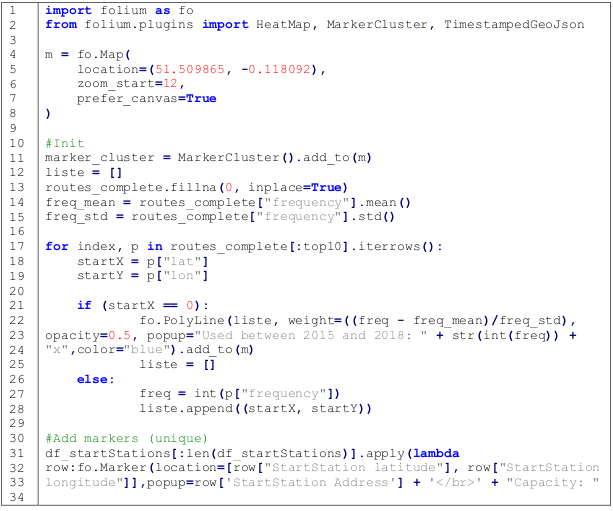
\includegraphics[width=1.2\textwidth]{img/listing1}\label{fig:listing1}
%\captionof{figure}{Result of \acs{mlp} with MinMaxScaler}\label{fig:listing1}
\end{figure}
\begin{figure}[H]
\hspace{-1.6cm}
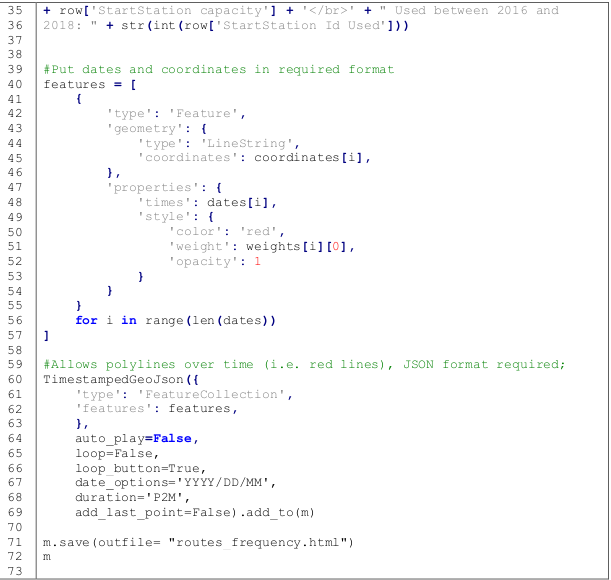
\includegraphics[width=1.2\textwidth]{img/listing2}\label{fig:listing2}
\captionof{figure}{Route usage over time plot}\label{fig:listing2}
\end{figure}
As the code from figure \ref{fig:listing2} shows, the poly lines on the map have been added iteratively. The
weight parameter can be used to determine the thickness of the poly line. Since these should look
as dynamic as possible on the map, the weight has been standardized. The fixed stations were
initially added, but no duplicate stations were plotted. A disadvantage of the plugin is that it needs
the data in a JSON format. Therefore the coordinates for the single points of a poly line as well as
the time series data had to be converted into a compatible format. As can be seen from the Python
code, the coordinates must be given the type \glqq LineString\grqq.  A LineString is defined as a sequence
of uniquely assignable points. In this case, the longitude and latitude previously requested using
the Graphhopper API on our Graphhopper server were sufficient. It is important that the parameter \glqq date\_options\grqq in \glqq TimestampedGeoJson\grqq corresponds exactly to the date format as in the nested
list dates, otherwise the time slider function on the map will not work properly.
Applied to the bicycle data the following picture results for the time 26.06.2016:
\begin{figure}[H]
%\hspace{-1.6cm}
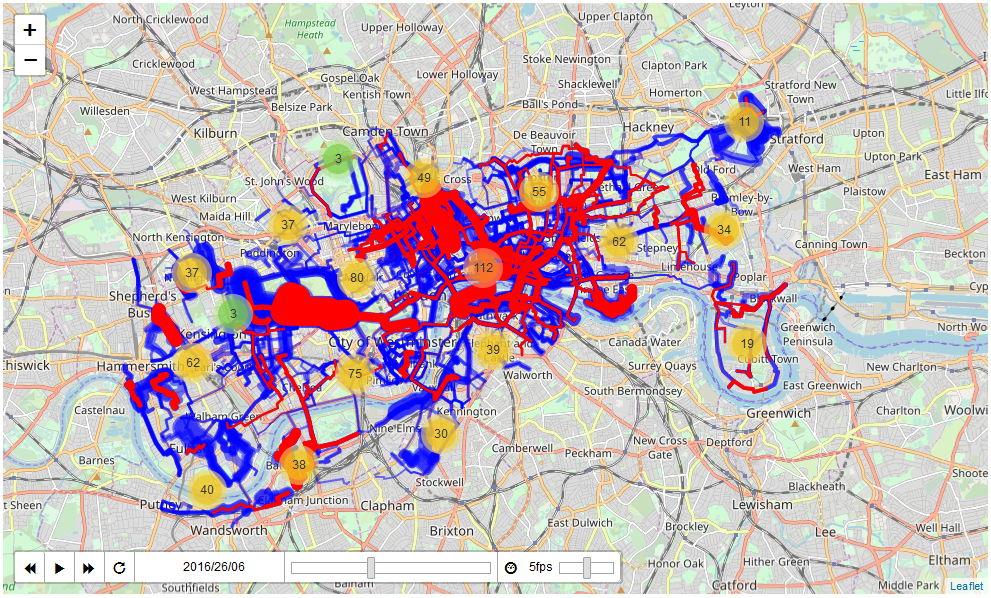
\includegraphics[width=1\textwidth]{img/figure4_folium_plot1}\label{fig:figure4_folium_plot1}
\captionof{figure}{Used bicycle routes over time plot (high usage)}\label{fig:figure4_folium_plot1}
\end{figure}
From figure \ref{fig:figure4_folium_plot1} it can be seen that on this day there was a moderate use of Santander Bicycles in
inner London. Especially the hubs such as Kings Cross or Hyde Park were obviously used very
often with Santander Bicycles on this spring day. Furthermore, the map with the thickness of the
poly lines shows how often this route was used in relation to the total use of all routes. The red
colored routes from figure \ref{fig:figure4_folium_plot1} are the actually used routes on this particular day, while the blue
routes are the \glqq inactive\grqq ones. The bubbles with the numbers represent the respective rental
stations. These have only been aggregated to provide a clearer representation. If the map is
zoomed in (figure \ref{fig:figure4_folium_plot1}), the granularity is refined and the markers of the individual rental station
locations are displayed. The color of these bubbles correlates with the number of aggregated
stations in the vicinity. This method also has the advantage that it is easy to see where most rental
stations are located. In fact, with 112 stations (see figure \ref{fig:figure4_folium_plot1}), the inner districts connected by the
Waterloo Bridge and the London Blackfriars Bridge form the center of most stations which are
close by. It should be noted, however, that new rental stations are constantly being added (even
given up again!), and a new data extract could result in a different picture. Therefore this assumption is valid for the selected date from figure \ref{fig:figure4_folium_plot1}, but not for today or in two years. A useful
feature that comes along with the folium plugin is the automatic data display sequence \cite{RN5}. When
someone clicks on the \glqq Play\grqq button from figure \ref{fig:figure4_folium_plot1}, all time series data is automatically run through.
The speed can be adjusted with the \glqq fps\grqq slider.
To give a counterexample, the following map shows the use of the routes on a winter’s day:
\begin{figure}[H]
%\hspace{-1.6cm}
\begin{center}
%\vspace{-0.9cm}
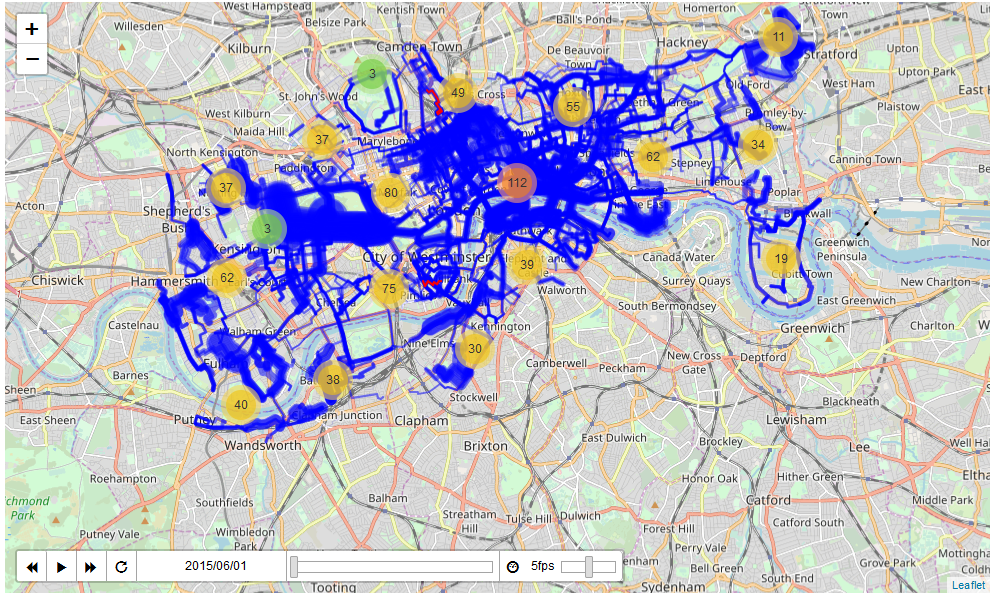
\includegraphics[width=1\textwidth]{img/figure5_folium_plot2}\label{fig:figure5_folium_plot2}
\captionof{figure}{Used bicycle routes over time plot (low usage)}\label{fig:figure5_folium_plot2}
\end{center}
\end{figure}
On 06.01.2015 obviously less bicycles were rented than in figure \ref{fig:figure4_folium_plot1}. This is due to the fact that at
this time it was winter and on the other hand there were only 315 Santander bicycle rental stations
all over London \cite{RN6}. In the course of time, new stations were added again and again, resulting in
a network which is monitored and managed by the local government and administrated by TfL.
The interactive map is also available on the \href{http://i-hadoop-01.informatik.hs-ulm.de/routes_frequency.html}{Hadoop Cluster}.
Overall, it can be observed that the usage of the rental stations has risen sharply on average over
the last four years. This can be explained by the expansion of the network but also by the increased
environmental awareness of the citizens. It is to be expected that further stations will be connected
in the future, so that ideally there will be one rental station at each crossroad in the town.
\subsection{Feature Engineering Kings Cross}\label{king}
Next, the features for the most frequently used station (Kings Cross) were prepared and
aggregated on a daily basis. In addition, these features have been extended by more like
\emph{Holidays, Weekdays, Months, Seasons} and weather data. This enrichment of the features
should help to achieve a higher accuracy of the learning model. For the weather data the weather
API \glqq Dark Sky\grqq was used. Like every available weather API the free use is limited. In the case of
Dark Sky a maximum of 1000 API request calls per day can be executed with one key \cite{RN7}.
However, this limitation can be bypassed if multiple accounts are used. Since each account has
a key, the keys can be collected and thus in fact significantly more requests can be executed.
However, this cannot be applied to the existing data sets of the bicycle data, since the daily
aggregated data of Kings Cross alone has already 376625 rows. Therefore a \glqq dates\grqq file was
created, which contains all days from 04.01.2015 - 14.04.2019 and thus covers all possible date
values of the rental station data. This has the advantage that now only 1562 API requests are
necessary and two keys are sufficient. The disadvantage of this method is that of course no precise
weather data can be retrieved at every station. Therefore the coordinates for the weather data of
the centroids (51.509865,-0.118092) of London were chosen. Dark Sky API also returns a JSON
file as response, which can be searched for the desired information. The following function from
the script \glqq Cycleusage \& Cycleroutes [allStations].ipynb\grqq shows the corresponding request call:
\begin{figure}[H]
\hspace{-1.6cm}
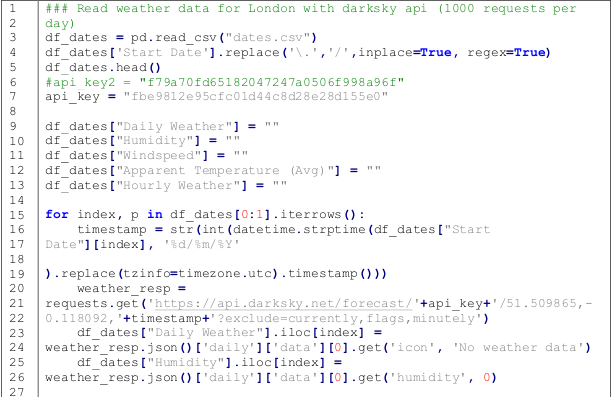
\includegraphics[width=1.2\textwidth]{img/listing3}\label{fig:listing3}
%\captionof{figure}{Result of \acs{mlp} with MinMaxScaler}\label{fig:listing1}
\end{figure}
\begin{figure}[H]
\hspace{-1.6cm}
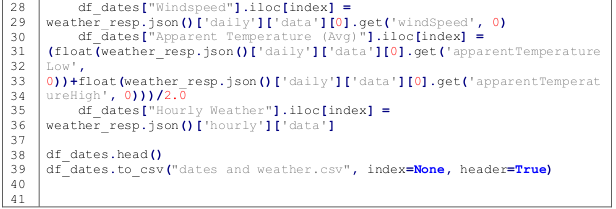
\includegraphics[width=1.2\textwidth]{img/listing4}\label{fig:listing4}
\captionof{figure}{Fetching the weather API with Python}\label{fig:listing4}
\end{figure}
As the code from figure \ref{fig:listing4} clearly shows, the following weather data were considered as relevant:
\glqq Daily Weather, Humidity, Windspeed\grqq and \glqq Apparent Temperature (Avg)\grqq . The feature \glqq Daily
weather\grqq returns a string value, how general the weather was on that particular day (e.g. sunny,
partly-cloudy...). Dark Sky makes this value dependent on the worst condition that occurred on
that day \cite{RN7}. That is, if it snowed for an hour, but the rest of the day was cloudy, \glqq Daily Weather\grqq will still show \glqq snowy\grqq  because this condition is weighted higher.\\\\
In addition to the weather data mentioned above, the hourly weather data of each day was also
queried as JSON lists, as otherwise every hour of each day would have to be queried separately,
which would drastically increase the API calls. A drawback of this variant is that the dates and
weather dataframe has a mixed structure. While the column \glqq hourly weather\grqq is a JSON format,
the other columns have a normal structure. This problem is further addressed in the section \glqq Data
Preparation - Hourly Base\grqq .\\\\
The processed weather data were next merged with the processed cycle usage dataframe. For
the Holidays the Python package \glqq holidays\grqq was used, which returns the corresponding holidays
to a selected location. Similarly, the features \emph{Weekdays, Months} and \emph{Seasons} were be
generated with defined functions and afterwards merged back with the main dataframe.\\\\
Subsequently, the dataframe was supplemented by \glqq past\grqq and\glqq future\grqq data. This should improve
the training of regression models, for example. A kind of \glqq sliding window\grqq was implemented for
the past data. This means that these columns always contain the value of the previous day. With
the future usage data, the daily number of borrowed bikes of the next day was also displayed. The
column \glqq Rented Bikes\grqq (i.e. usage) corresponds to the class variable of interest. This has the
consequence that the first and last day in the dataframe have missing values, because there is no
data for this naturally. The prepared dataframe for Kings Cross on a daily basis looks after the
preparation steps like this:
\begin{figure}[H]
\hspace{-2.8cm}
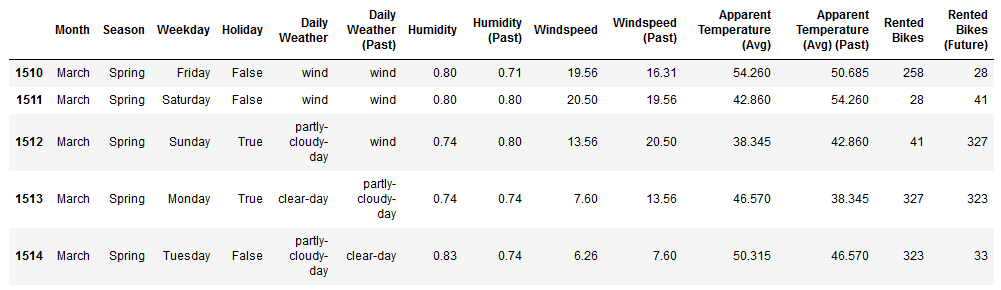
\includegraphics[width=1.4\textwidth]{img/figure6_kings_cross_df}\label{fig:figure6_kings_cross_df}
\captionof{figure}{Prepared data frame of Kings Cross (daily)}\label{fig:figure6_kings_cross_df}
\end{figure}
As one can see from figure \ref{fig:figure6_kings_cross_df}, the past data was only included for the weather data whereas the
future data was only added for the usage of the rental station. The string values were later be
transformed into numerical values since machine learning methods always require number values
instead of string values. Therefore a proper schema was defined, which is described in more detail
in the modeling section.\\\\
With the processed bicycle data from \ref{fig:figure6_kings_cross_df}, machine learning can already be used to predict,
for example, the daily usage of bicycles (i.e. how many bicycles will be borrowed tomorrow starting
from today?). The script \glqq Feature Engineering Kings Cross.ipynb\grqq contains the preparation
functions described above and can be found on our GitHub repository.
\subsection{Data Prediction with MLPRegressor}\label{sec:mlp}
Since we wanted to implement the prediction algorithm in Python we used the library \emph{Scikit Learn} which provides a class \emph{\acf{mlp}} with according functions.
As we wanted to train a non-linear model we decided to use a Multi-layer Perceptron since it can learn a non-linear function approximator for either classification or regression. However  the \acs{mlp} uses backpropagation which is the most widely used algorithm for supervised learning with multi-layered feed-forward networks \cite{riedmiller1993direct}, this algorithm was implemented to train a prediction model for the rental bike usage on a daily base.\\\\
The outcome of of the Data Profiling Part 2, as described in chapter \ref{sec:dp2} served as a basis for the prediction.
As a first implementation we used the following data as an input for the feature matrix: \emph{Month, Weekday, Day, Season, Daily Weather, Daily Weather Past, Humidity, Humidity Past, Windspeed, Windspeed Past, Apparent Temperature (Avg), Apparent Temperature (Avg) Past, Rented Bikes}. Since we assume that weather conditions play an important role in bike usage we decided to add weather data. Another assumption was that on weekdays the frequency will rise, because a lot of people use rented bikes to travel to work. Furthermore we added the number of rentals of today in order to predict the ones of tomorrow. Therefore \emph{Rented Bikes Future} served as our target variable which is to predicted.\\
Since the \acs{mlp} works with data represented as dense and sparse numpy arrays of floating point values, data had to be encoded accordingly beforehand. Therefore we mapped all of the ordinal scaled data like \emph{Month, Weekday, Season, Daily Weather} to numerical data, by implementing a dictionary which assigns numerical values to ordinal data. E. g. For the weekdays we used the following dictionary:
\begin{lstlisting}[language=bash,breaklines=true]
"Weekday": {"Monday": 1, "Tuesday": 2, "Wednesday": 3, "Thursday": 4,"Friday": 5, "Saturday": 6, "Sunday":7 }
\end{lstlisting}
After the encoding we split the data into 80 \% training data and 20\% test data.
Since the \acs{mlp} is sensitive to feature scaling we normalized the data accordingly to the activation function. Since we used the \emph{logistic} activation function which expects values between [0,1] we normalized the feature matrix as well as the target variable beforehand. Scikit Learn provides several scaling mechanism to rescale the data. 
After data was scaled we applied the \acs{mlp} with \emph{logistic} as an activation function and ten hidden layers with five neurons. After the prediction we denormalized the data back to its original state. In order to rate the accuracy of the prediction we computed the \acf{rmse} which measures the difference between actual and predicted values of a model. The less the difference respectively the value, the better is the model.
To get a better impression of how the prediction worked, the results were plotted as time series.
The time series was plotted over for years, which causes the plot to be very large. In order to make it more user friendly, we implemented an interactive plot which gives the user the opportunity to zoom into specific parts or cut out some parts to look at them more closely.
\subsubsection{Normalization}\label{sec:normalization}
In the first attempt we used the \emph{MinMaxScaler} which rescales the data such that all vales are in the range of [0,1].
This gave us a \acs{rmse} of 122.347. To get a better impression of what that means we plotted this result which can be seen in figure \ref{fig:mlpquantile}.
\begin{figure}[H]
\hspace{-2.8cm}
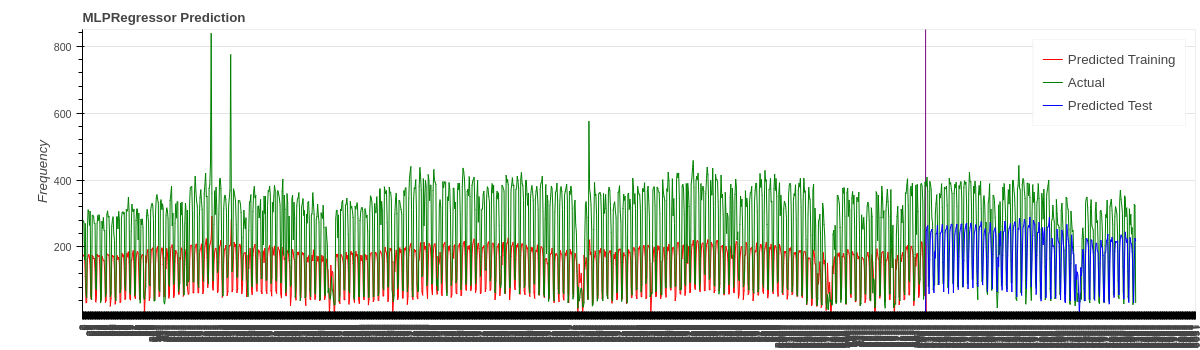
\includegraphics[width=1.4\textwidth]{img/mlpminmax}\label{fig:mlpminmax}
\captionof{figure}{Result of \acs{mlp} with MinMaxScaler}\label{fig:mlpminmax}
\end{figure}
This result shows that the prediction lack accuracy. As we found out this was caused by the MinMaxScaler, since this scaler is very sensitive to the presence of outliers. Therefore we chose another scaler for normalization which is more prone to outliers. In order to find a more suitable scaler, experiments were made with all available scalers of Scikit Learn which met the requirements for the output of the scaling. The best result was achieved by the \emph{QuantileTransformer} with a \acs{rmse} of 57.837, therefore we stuck with this normalization method.
\subsubsection{Feature Evaluation}\label{sec:featureeval}
In order to improve accuracy, further experiments were carried out to evaluate the features. As mentioned earlier the previous predictions were made with a feature matrix of thirteen features. To evaluate which features improve the prediction and which are useless 18 test cases were carried out. Each test case consists of different constellations of features. In the end the different \acs{rmse} values were compared, which can be seen in figure \ref{fig:evalmlp}.
\begin{figure}[H]
\hspace{-1.5cm}
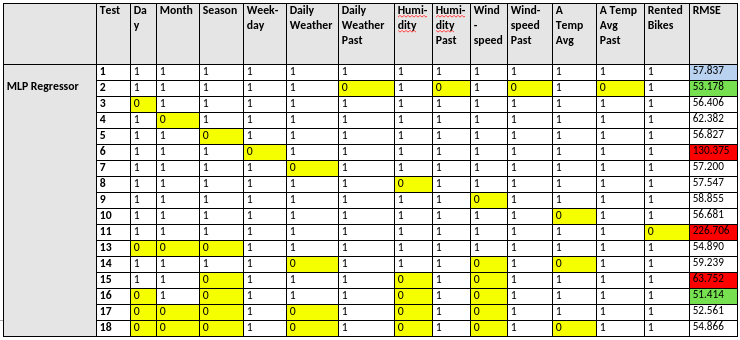
\includegraphics[width=1.2\textwidth]{img/evalmlp}\label{fig:evalmlp}
\captionof{figure}{Feature evaluation test cases}\label{fig:evalmlp}
\end{figure}
Figure \ref{fig:evalmlp} shows beneath the different test cases, included features, those are assigned to \glqq 1\grqq
 and excluded features which are assigned to \glqq 0\grqq. The first \acs{rmse} value, colored in blue depicts the prediction accuracy with all 13 features. The red colored values show the constellations which are significantly worse than the original one and in turn the green values represent the values with an increased accuracy than the original one.
\subsubsection{Result}\label{sec:resultmlp}
This evaluation showed that the features \emph{Weekday} and \emph{Rented Bikes} are the most important ones and in turn the features \emph{Day} and \emph{Season} are less important.
Based on our testing results we recommend to use the following nine features: \emph{Weekday, Month, Past Data, Apparent Temperature (Avg), Daily Weather} and \emph{Rented Bikes}. 
Moreover experiments with scalers showed that the \emph{QuantileTransformer} is more prone to outliers than others and is therefore the scaler of choice.\\
First plots were made with the library \emph{Matplotlib} which turns out to be very restricted and complicated to handle in order to create interactive plots. Therefore we recommend to use \emph{Bokeh} which provides easy to implement interactive plots especially for large data sets.\\
Applying the recommendations regarding scaling and feature evaluation we received a \acs{rmse} value of 51.414 which is the best value achieved during the project phase. The overall result visualized with \emph{Bokeh} can be seen in figure \ref{fig:mlpquantile}.
\begin{figure}[H]
\hspace{-2.8cm}
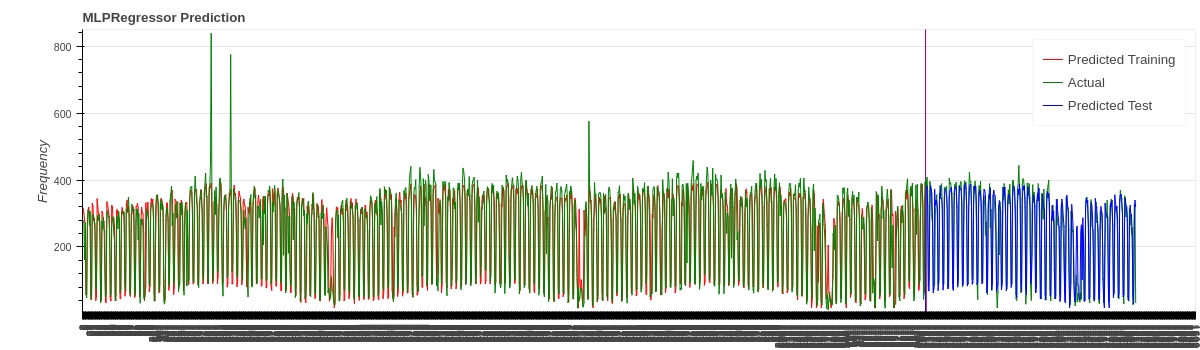
\includegraphics[width=1.4\textwidth]{img/mlpquantile}\label{fig:mlpquantile}
\captionof{figure}{Accuracy with recommended features and scaling by the QuantileTransformer}\label{fig:mlpquantile}
\end{figure}
Compared to figure \ref{fig:mlpminmax} one can see significant improvements in accuracy.\\
This model is based on the most used station, which is King´s Cross with a dataset of 1515 records. In order to confirm this model we applied it to the least used station in Farringdon Street, Holborn as well. The result can be seen in figure  \ref{fig:mlpquantile_least}.
\begin{figure}[H]
\hspace{-2.8cm}
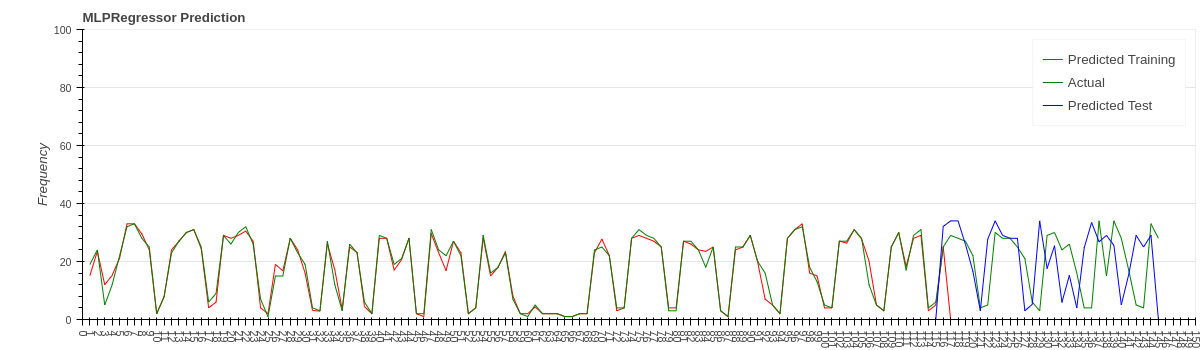
\includegraphics[width=1.4\textwidth]{img/mlpquantile_least}\label{fig:mlpquantile_least}
\captionof{figure}{Accuracy with recommended features and scaling by the QuantileTransformer}\label{fig:mlpquantile_least}
\end{figure}
The accuracy of the prediction of the least used station measures a \acs{rmse} of 9.311. This shows that the model works not only for highly frequented stations but also for stations like Farringdon Street with only 145 records.
\subsection{Data Prediction with Spark}\label{sec:spark}
Apache Spark's \acf{mlib} is designed for simplicity, scalability, and easy
integration with other tools. With the scalability, language compatibility, and speed of Spark,
data scientists can focus on their data problems and models instead of solving the complexities
surrounding distributed data (such as infrastructure, configurations, and so on).
Built on top of Spark, MLlib is a scalable machine learning library consisting of common learning
algorithms and utilities, including classification, regression, clustering, collaborative filtering,
dimensionality reduction, and underlying optimization primitives. Spark MLlib seamlessly
integrates with other Spark components such as Spark SQL, Spark Streaming, and DataFrames
and is installed in the Databricks runtime. The library is usable in Java, Scala, and Python as
part of Spark applications, so that you can include it in complete workflows.
MLlib allows for preprocessing, munging, training of models, and making predictions at scale on
data. You can even use models trained in MLlib to make predictions in Structured Streaming.
Spark provides a sophisticated machine learning API for performing a variety of machine
learning tasks, from classification to regression, clustering to deep learning \cite{Databricks2019}.\\\\
MLlib is Spark’s scalable machine learning library consisting of common learning algorithms and
utilities that can be divided into two categories:\\\\
Supervised learning:
\begin{itemize}
\item Classification and regression
\begin{itemize}
\item naive Bayes
\item linear models (SVMs, logistic regression, linear regression)
\item decision trees
\item ensembles of trees (Random Forests and Gradient-Boosted Trees)
\end{itemize}
\end{itemize}
Unsupervised learning:
\begin{itemize}
\item Collaborative filtering
\begin{itemize}
\item \acf{als}
\end{itemize}
\item Clustering
\begin{itemize}
\item k-means
\end{itemize}
\item Dimensionality reduction
\begin{itemize}
\item \acf{pca}
\item \acf{svd}
\end{itemize}
\end{itemize}
Spark 1.2 includes a new package called spark.ml, which aims to provide a uniform set of
high-level APIs that help users create and tune practical machine learning pipelines. It is
currently an alpha component, and we would like to hear back from the community about how it
fits real-world use cases and how it could be improved.
\subsubsection{Selected Algorithms}\label{sec:sparkalgos}
Regression analysis consists of a set of machine learning methods that allow us to predict a
continuous outcome variable (y) based on the value of one or multiple predictor variables (x).
Since our goal is to make predictions on a continuous feature, the next step is to implement the
algorithms provided the library and compare their results.\\\\

\textbf{Decision Tree Regression}\\\\

A decision tree is built top-down from a root node and involves partitioning the data into subsets
that contain instances with similar values (homogeneous). We use standard deviation to calculate
the homogeneity of a numerical sample. If the numerical sample is completely homogeneous its
standard deviation is zero \cite{Saed2019}.
\begin{figure}[H]
\centering
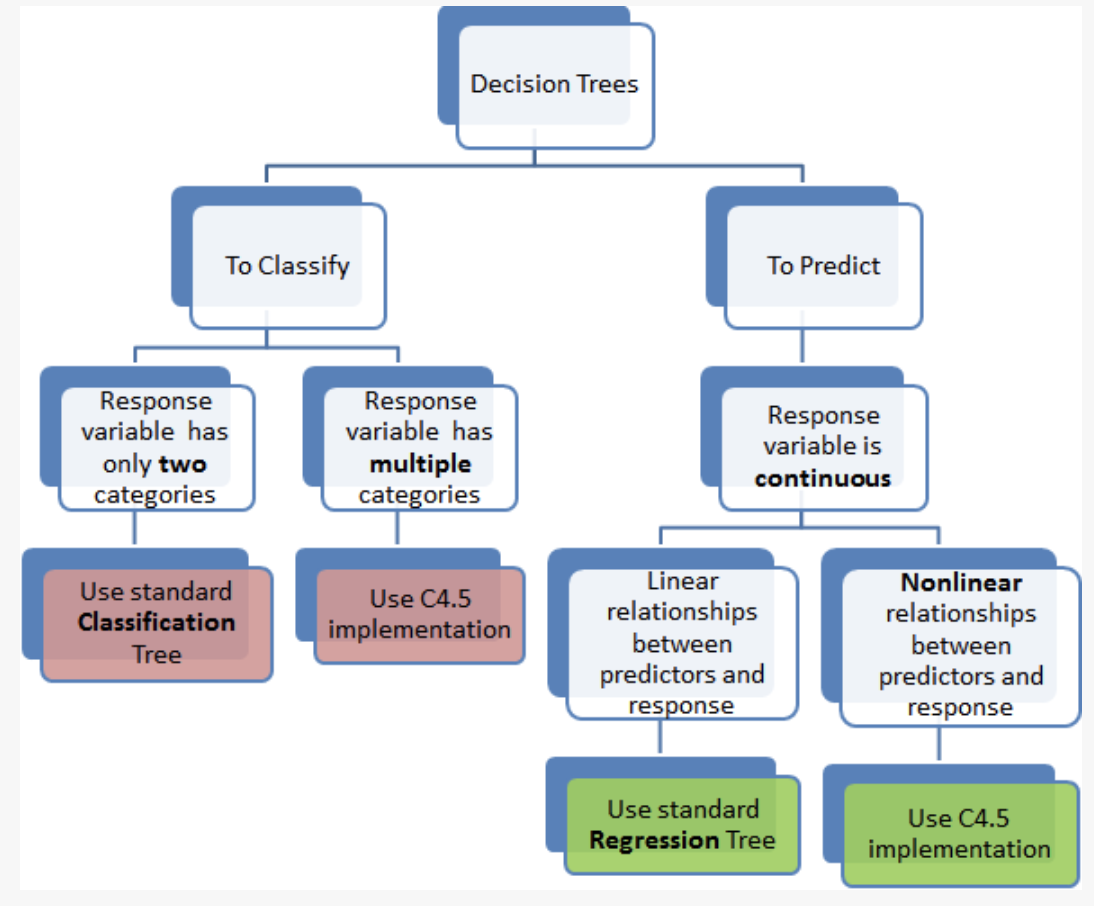
\includegraphics[width=0.8\textwidth]{media/dt}\label{fig:dt}
\captionof{figure}{Decision tree usage diagram}\label{fig:dt}
\end{figure}
In a standard classification tree, the idea is to split the dataset based on homogeneity of data.
Lets say for example we have two variables: age and weight that predict if a person is going to
sign up for a gym membership or not. In our training data if it showed that 90\% of the people
who are older than 40 signed up, we split the data here and age becomes a top node in the
tree. We can almost say that this split has made the data "90\% pure". Rigorous measures of
impurity, based on computing proportion of the data that belong to a class, such as entropy or
Gini index are used to quantify the homogeneity in Classification trees \cite{BalaDeshpande2011}.
In a regression tree the idea is this: since the target variable does not have classes, we fit a
regression model to the target variable using each of the independent variables. Then for each
independent variable, the data is split at several split points. At each split point, the "error"
between the predicted value and the actual values is squared to get a \acf{sse}. The split point errors across the variables are compared and the variable/point yielding
the lowest SSE is chosen as the root node/split point. This process is recursively continued \cite{BalaDeshpande2011}.\\\\
Regression trees are needed when the response variable is numeric or continuous. For
example, the predicted price of a consumer good. Thus regression trees are applicable for
prediction type of problems as opposed to classification.
Keep in mind that in either case, the predictors or independent variables may be categorical or
numeric. It is the target variable that determines the type of decision tree needed \cite{BalaDeshpande2011}.\\\\

\textbf{Random Forest Regression}\\\\
A Random Forest is an ensemble technique capable of performing both regression and
classification tasks with the use of multiple decision trees and a technique called Bootstrap
Aggregation, commonly known as bagging. What is bagging you may ask? Bagging, in the
Random Forest method, involves training each decision tree on a different data sample where
sampling is done with replacement.
\begin{figure}[H]
\centering
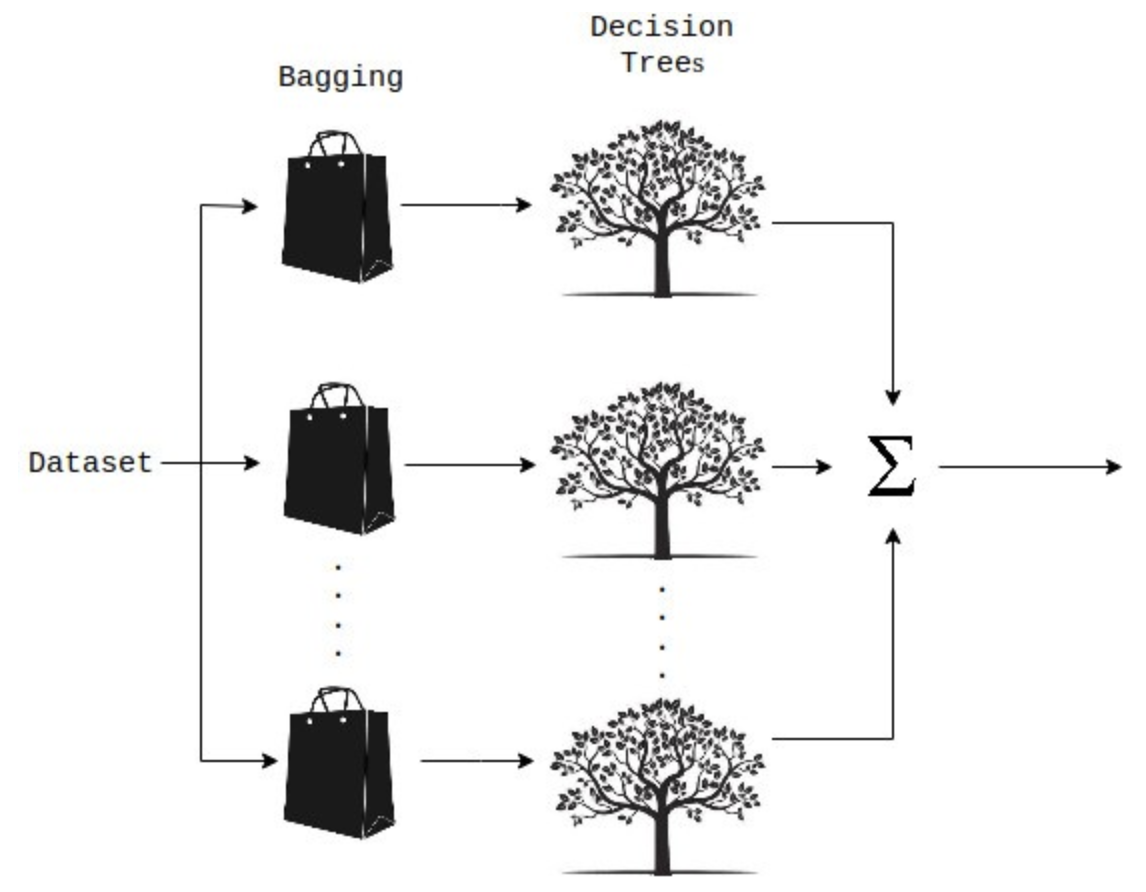
\includegraphics[width=0.8\textwidth]{media/rf}\label{fig:rf}
\captionof{figure}{Random Forest Regression: Process}\label{fig:rf}
\end{figure}
The basic idea behind this is to combine multiple decision trees in determining the final output
rather than relying on individual decision trees. If you want to read more on Random Forests, I
have included some reference links which provide in depth explanations on this topic.\\\\

\textbf{Gradient Boosted Tree Regression}\\\\
The idea of boosting came out of the idea of whether a weak learner can be modified to become
better. Hypothesis boosting was the idea of filtering observations, leaving those observations
that the weak learner can handle and focusing on developing new weak learns to handle the
remaining difficult observations \cite{Brownlee2016}.\\\\
Gradient boosting involves three elements:\\
\begin{itemize}
\item A loss function to be optimized:The loss function used depends on the type of problem
being solved. It must be differentiable, but many standard loss functions are supported
and you can define your own.
\item A weak learner to make predictions: Decision trees are used as the weak learner in
gradient boosting. Specifically regression trees are used that output real values for splits
and whose output can be added together, allowing subsequent models outputs to be
added and “correct” the residuals in the predictions. Trees are constructed in a greedy
manner, choosing the best split points based on purity scores like Gini or to minimize the
loss. Initially, such as in the case of AdaBoost, very short decision trees were used that
only had a single split, called a decision stump. Larger trees can be used generally with
4-to-8 levels. It is common to constrain the weak learners in specific ways, such as a
maximum number of layers, nodes, splits or leaf nodes. This is to ensure that the
learners remain weak, but can still be constructed in a greedy manner.
\item An additive model to add weak learners to minimize the loss function: Trees are added
one at a time, and existing trees in the model are not changed. A gradient descent
procedure is used to minimize the loss when adding trees. Traditionally, gradient descent
is used to minimize a set of parameters, such as the coefficients in a regression equation
or weights in a neural network. After calculating error or loss, the weights are updated to
minimize that error. Instead of parameters, we have weak learner sub-models or more
specifically decision trees. After calculating the loss, to perform the gradient descent
procedure, we must add a tree to the model that reduces the loss (i.e. follow the gradient). We do this by parameterizing the tree, then modify the parameters of the tree
and move in the right direction by (reducing the residual loss.Generally this approach is
called functional gradient descent or gradient descent with functions \cite{Brownlee2016}.
\end{itemize}
\subsubsection{Implementation}\label{sec:sparkimpl}
The first step is to apply the algorithm using all the features, then each time based on the
features importance function, try to remove the least important columns and check for
improvements in the RMSE value.
The result of the testing process is described each step by a features importance plot. The
results are as well listed on a table.
The figures below show the correlation between the predicted data and the real future
measured data. The first test series was implemented by regarding the most used station.\\\\
\textbf{Decision Tree}\\
We start by generating a model considering all the features with a RMSE of 71.35.
\begin{figure}[H]
\centering
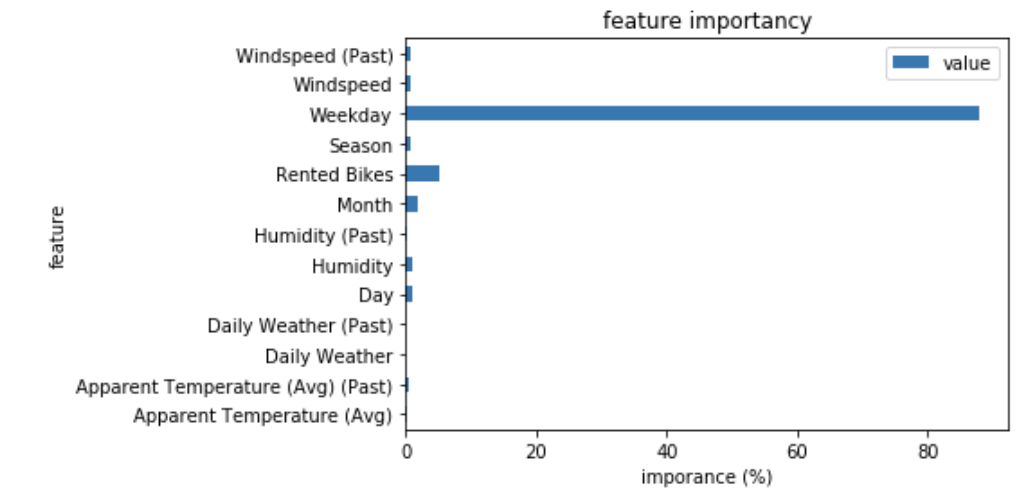
\includegraphics[width=0.8\textwidth]{media/test1_dt}\label{fig:test1_dt}
\captionof{figure}{Test 1 features importance: 71.35}\label{fig:test1_dt}
\end{figure}
Figure \ref{fig:anasst1} shows the removed columns and RMSE results on on each test:
The choice of removing features is explained by the features importance plots.
\begin{figure}[H]
\centering
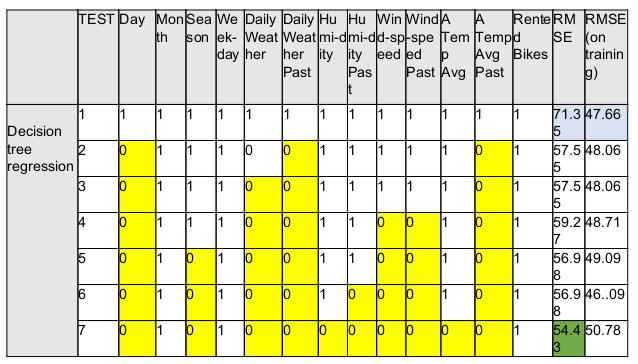
\includegraphics[width=0.8\textwidth]{media/anasst1}\label{fig:anasst1}
\captionof{figure}{Feature evaluation test cases}\label{fig:anasst1}
\end{figure}
\begin{figure}[H]
\centering
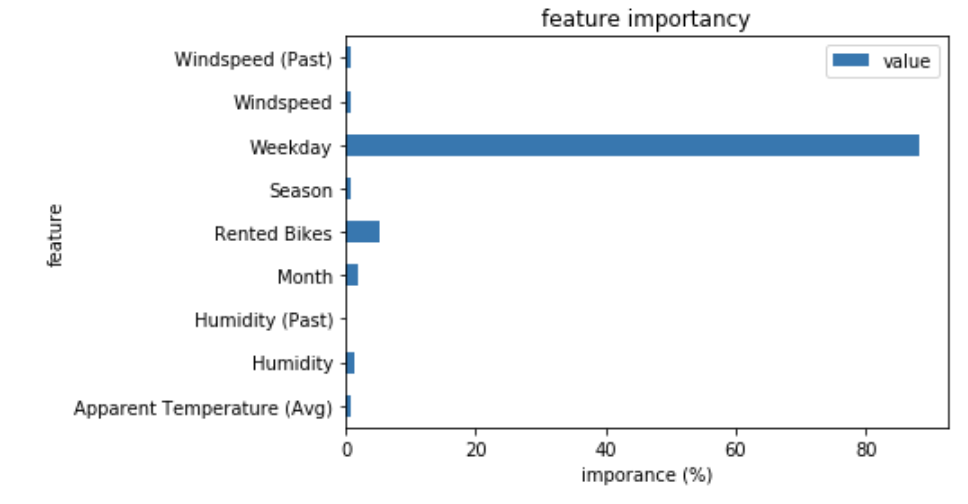
\includegraphics[width=0.8\textwidth]{media/test3_dt}\label{fig:test3_dt}
\captionof{figure}{Test 3 features importance: 57.55}\label{fig:test3_dt}
\end{figure}
\begin{figure}[H]
\centering
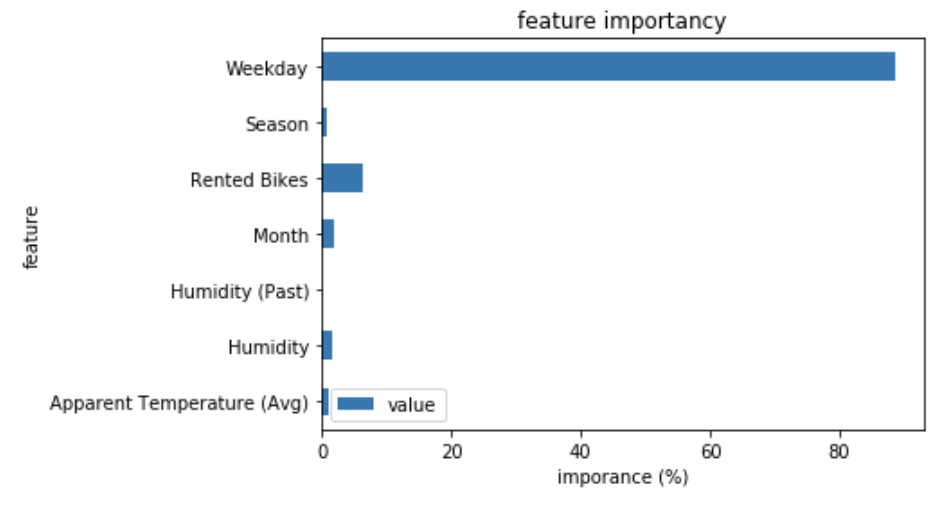
\includegraphics[width=0.8\textwidth]{media/test4_dt}\label{fig:test4_dt}
\captionof{figure}{Test 4​ features importance: 59.27}\label{fig:test4_dt}
\end{figure}
\begin{figure}[H]
\centering
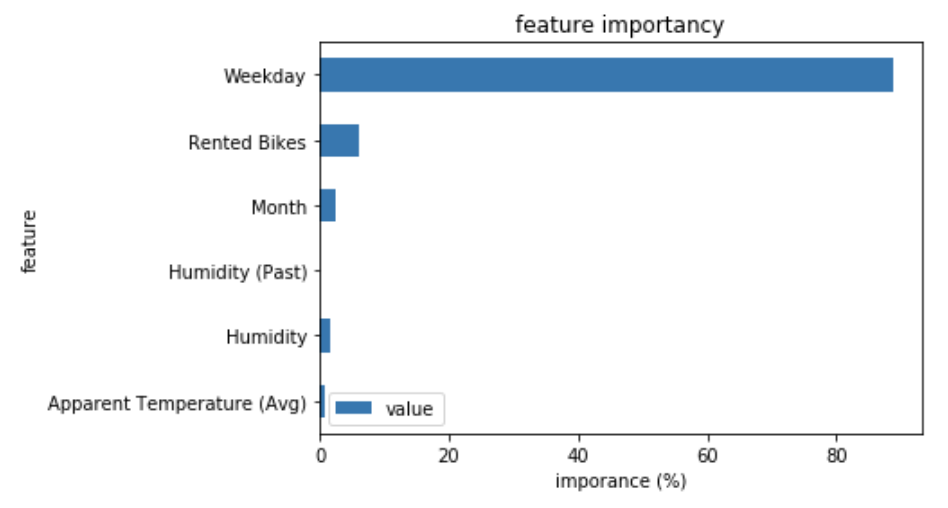
\includegraphics[width=0.8\textwidth]{media/test5_dt}\label{fig:test5_dt}
\captionof{figure}{Test 5​ features importance: 56.98}\label{fig:test5_dt}
\end{figure}
\begin{figure}[H]
\centering
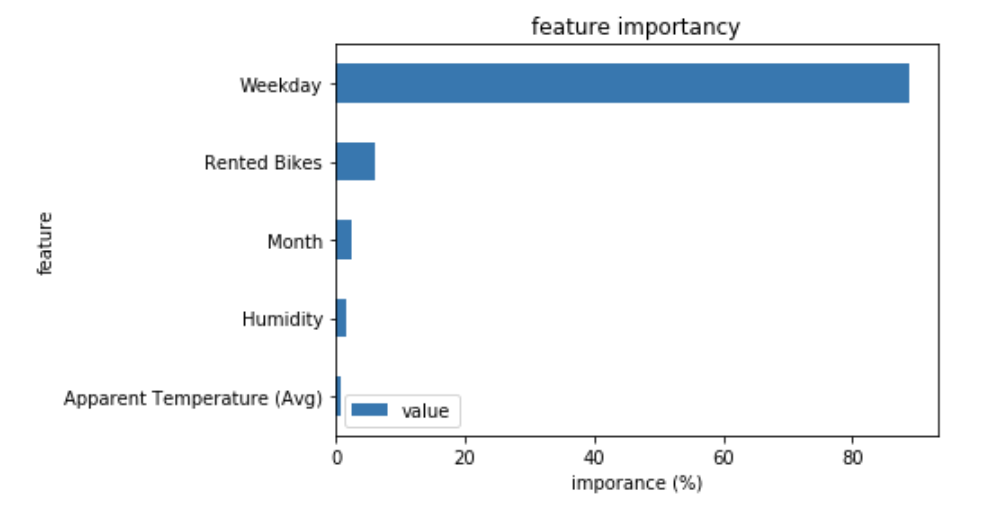
\includegraphics[width=0.8\textwidth]{media/test6_dt}\label{fig:test6_dt}
\captionof{figure}{Test 6​ features importance: 56.98}\label{fig:test6_dt}
\end{figure}
\begin{figure}[H]
\centering
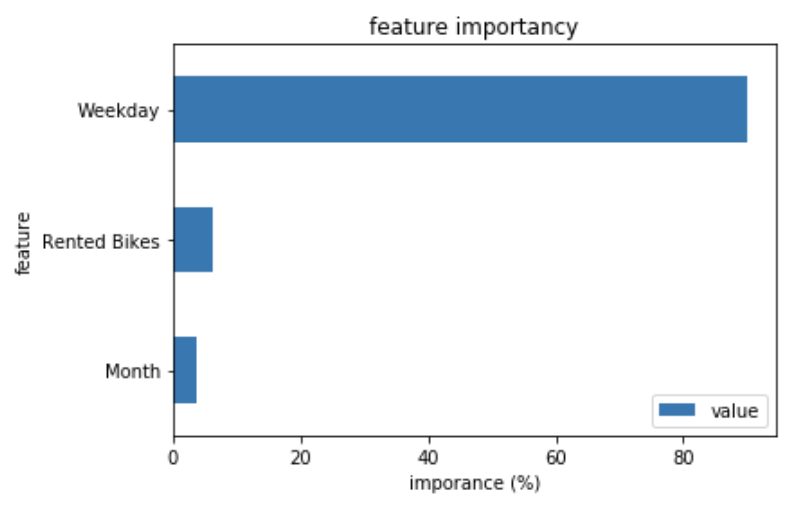
\includegraphics[width=0.8\textwidth]{media/test7_dt}\label{fig:test7_dt}
\captionof{figure}{Test 7​ features importance: 54.43}\label{fig:test7_dt}
\end{figure}
The final correlation results are shown in figure \ref{fig:image25} with an RMSE of 54.43.
\begin{figure}[H]
\centering
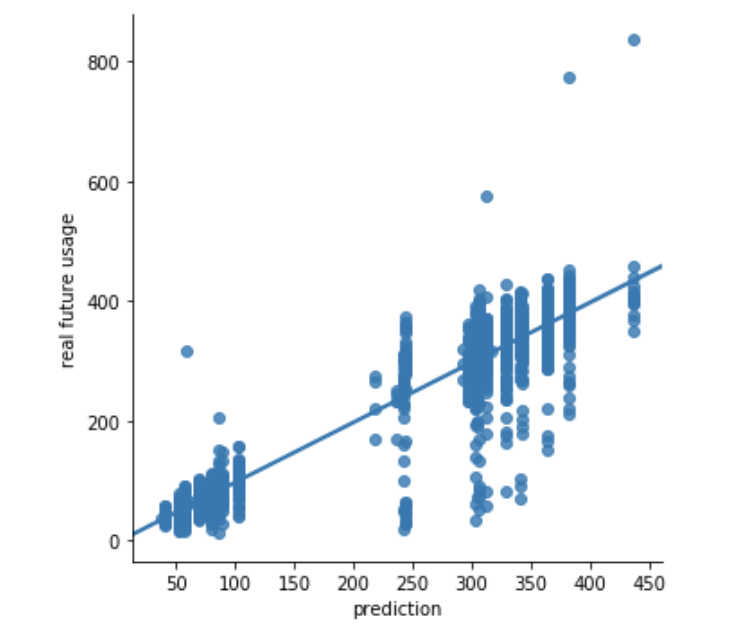
\includegraphics[width=0.6\textwidth]{media/image25}\label{fig:image25}
\captionof{figure}{Data distribution of the actual and predicted data bike usage using​ Decision Tree}\label{fig:image25}
\end{figure}
\begin{figure}[H]
\centering
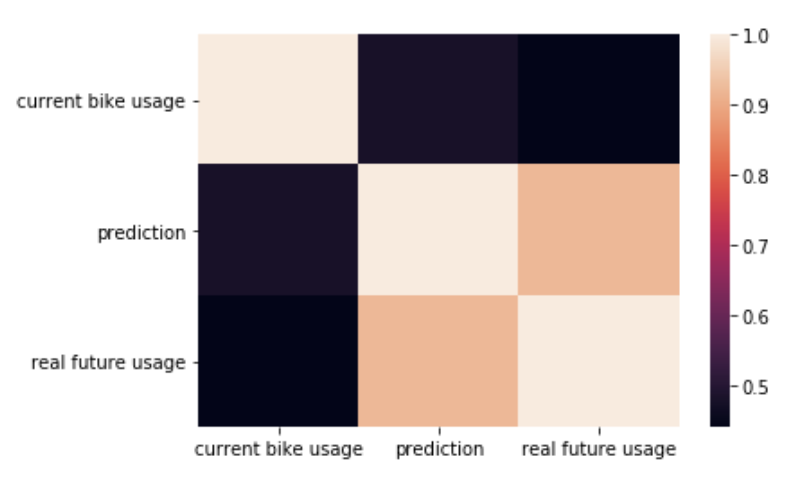
\includegraphics[width=0.8\textwidth]{media/image26}\label{fig:image26}
\captionof{figure}{Heat map correlation plot showing interval value of the regression line​ (Decision Tree)}\label{fig:image26}
\end{figure}
\textbf{Random Forest}\\
We start by generating a model considering all the features with a RMSE of 60.04.
\begin{figure}[H]
\centering
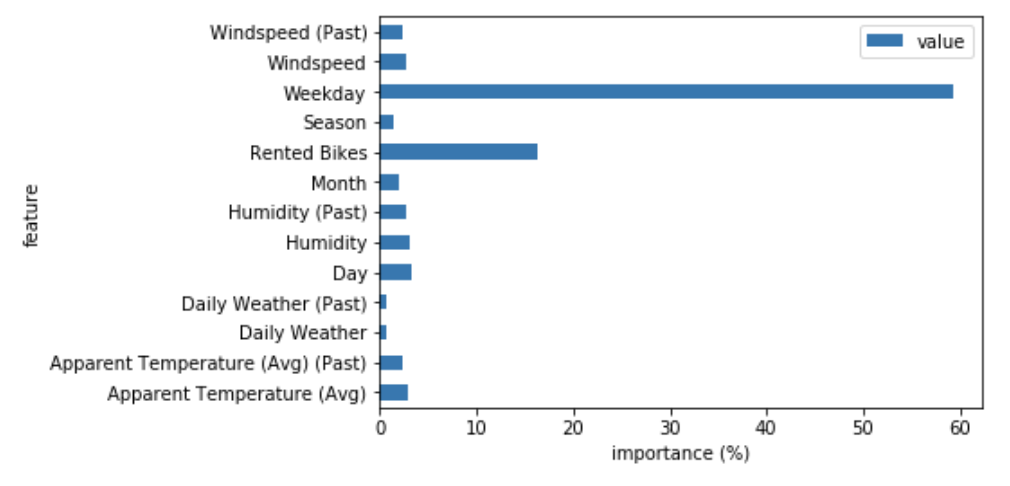
\includegraphics[width=0.8\textwidth]{media/test1_rd}\label{fig:test1_rd}
\captionof{figure}{Test ​1​ features importance: 60.04}\label{fig:test1_rd}
\end{figure}
Figure \ref{fig:anasst2} shows the removed columns and RMSE results on on each test:
The choice of removing features is explained by the features importance plots.
\begin{figure}[H]
\centering
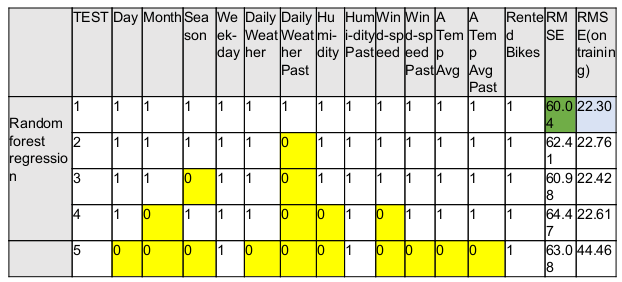
\includegraphics[width=0.8\textwidth]{media/anasst2}\label{fig:anasst2}
\captionof{figure}{Feature evaluation test cases}\label{fig:anasst2}
\end{figure}
The process consists of removing after each test the features with the least importance.
\begin{figure}[H]
\centering
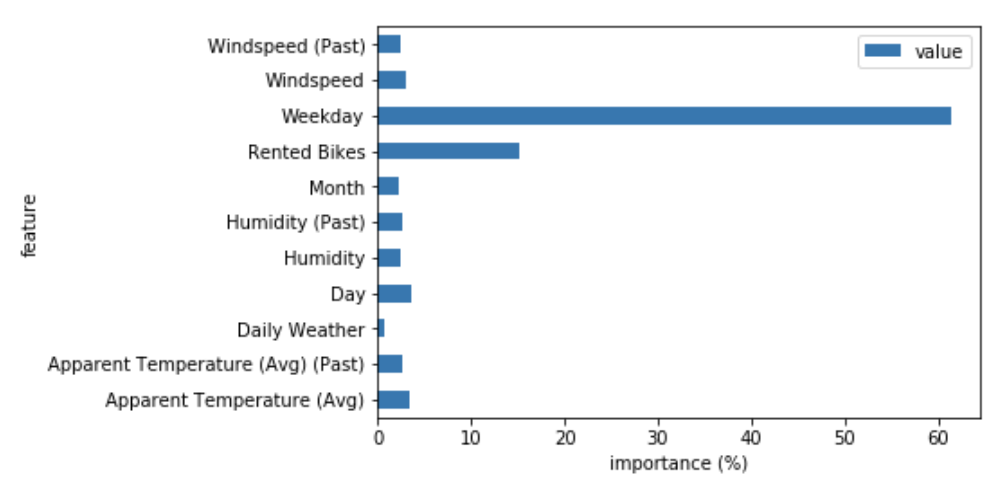
\includegraphics[width=0.8\textwidth]{media/test2_rd}\label{fig:test2_rd}
\captionof{figure}{Test ​2​ features importance: 62.41}\label{fig:test2_rd}
\end{figure}
\begin{figure}[H]
\centering
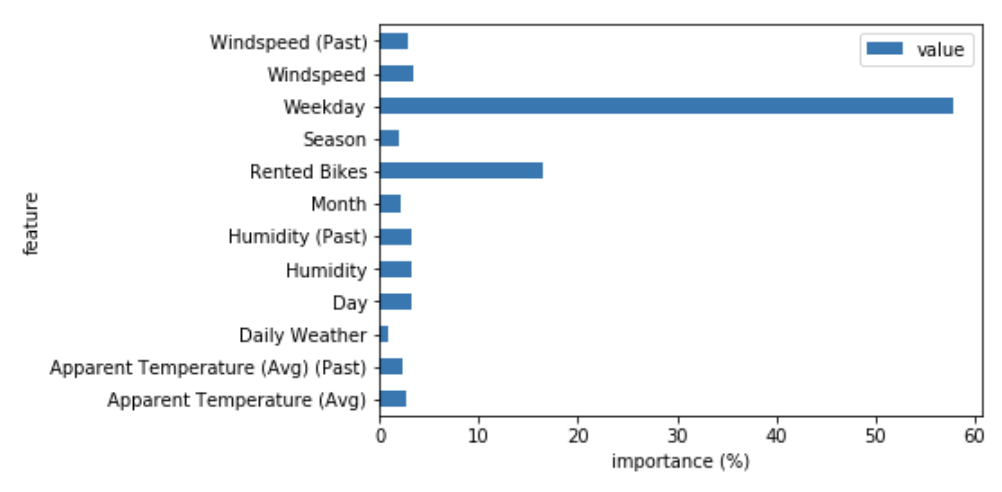
\includegraphics[width=0.8\textwidth]{media/test3_rd}\label{fig:test3_rd}
\captionof{figure}{Test ​3​ features importance: 60.98}\label{fig:test3_rd}
\end{figure}
\begin{figure}[H]
\centering
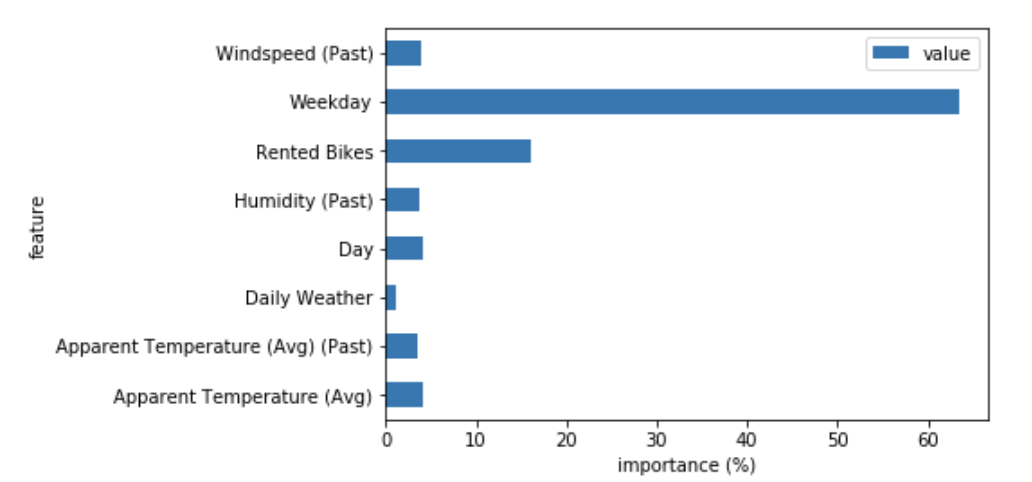
\includegraphics[width=0.8\textwidth]{media/test4_rd}\label{fig:test4_rd}
\captionof{figure}{Test 4 features importance: 64.64}\label{fig:test4_rd}
\end{figure}
\begin{figure}[H]
\centering
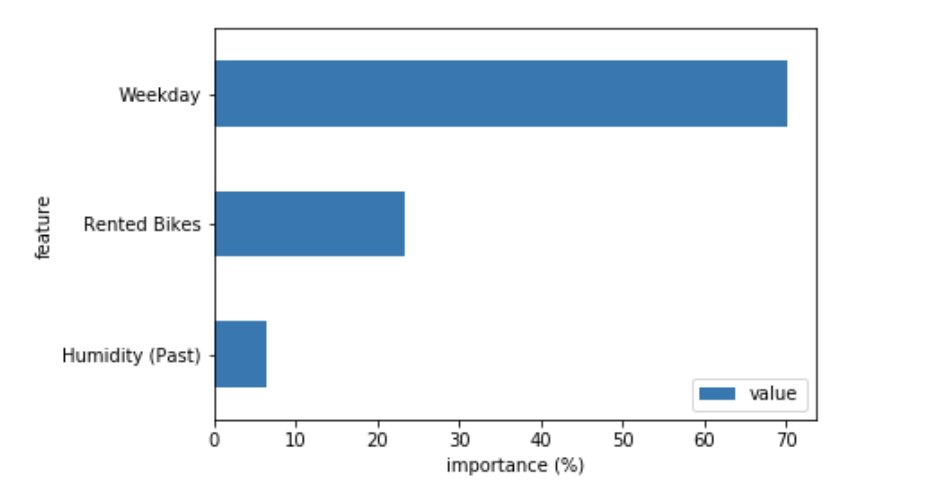
\includegraphics[width=0.8\textwidth]{media/test5_rd}\label{fig:test5_rd}
\captionof{figure}{Test 5 features importance: 63.08}\label{fig:test5_rd}
\end{figure}
The final correlation results are shown in figure \ref{fig:image2d} with an RMSE of 54.43.
\begin{figure}[H]
\centering
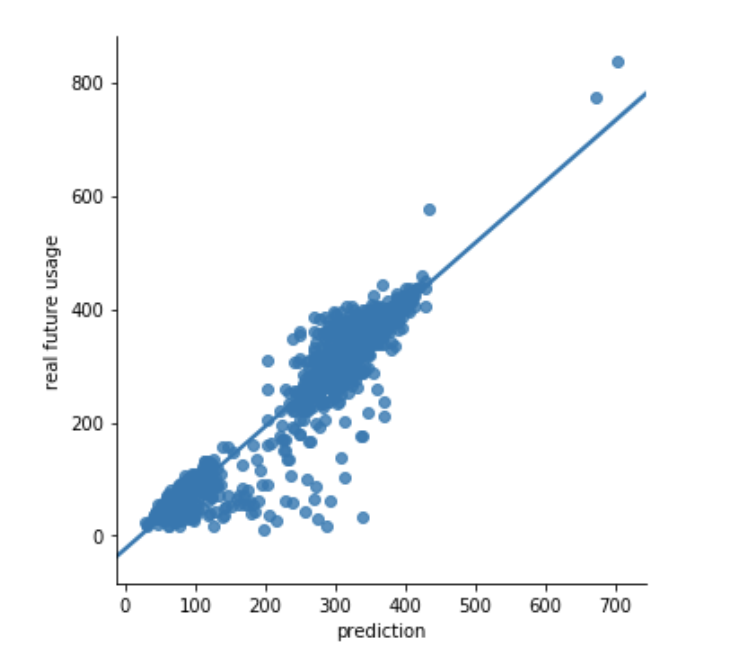
\includegraphics[width=0.6\textwidth]{media/image2d}\label{fig:image2d}
\captionof{figure}{Data distribution of the actual and predicted data bike usage using​ Random Forest}\label{fig:image2d}
\end{figure}
\begin{figure}[H]
\centering
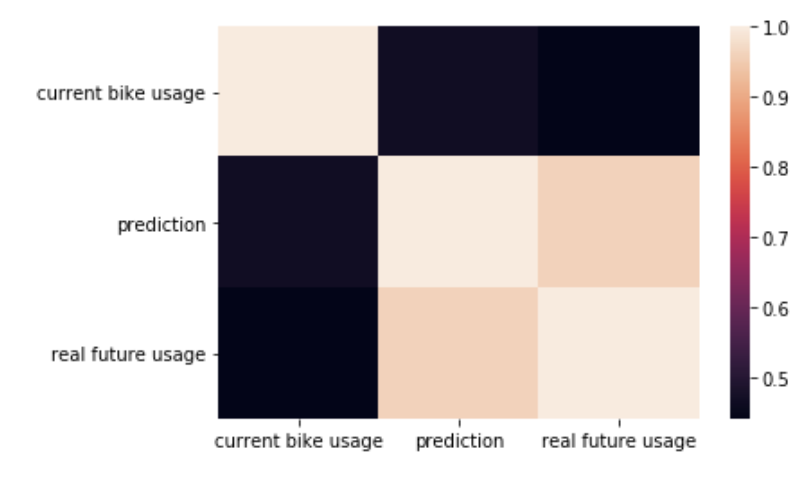
\includegraphics[width=0.8\textwidth]{media/image2e}\label{fig:image2e}
\captionof{figure}{Heat map correlation plot showing interval value of the regression line​ (Random Forest)}\label{fig:image2e}
\end{figure}

\textbf{Gradient boosted tree regression}\\
We start by generating a model considering all the features with a RMSE of 81.30.
\begin{figure}[H]
\centering
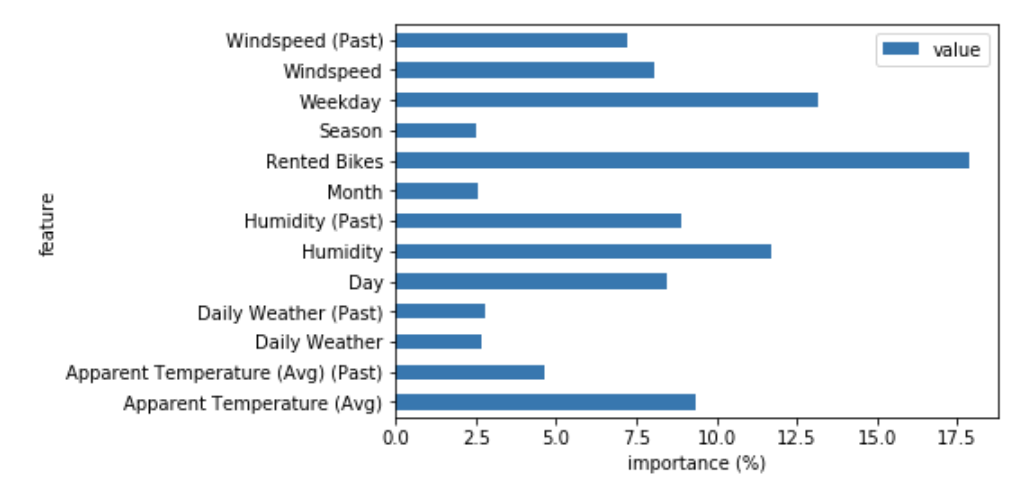
\includegraphics[width=0.8\textwidth]{media/test1_gb}\label{fig:test1_gb}
\captionof{figure}{Test ​1​ features importance: 81.30}\label{fig:test1_gb}
\end{figure}
Figure \ref{fig:anasst1} shows the removed columns and RMSE results on on each test:
The choice of removing features is explained by the features importance plots.
\begin{figure}[H]
\centering
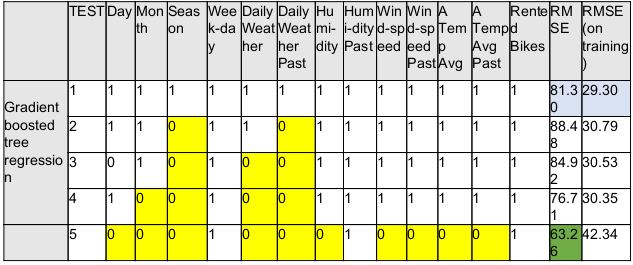
\includegraphics[width=0.8\textwidth]{media/anasst3}\label{fig:anasst3}
\captionof{figure}{Feature evaluation test cases}\label{fig:anasst3}
\end{figure}
\begin{figure}[H]
\centering
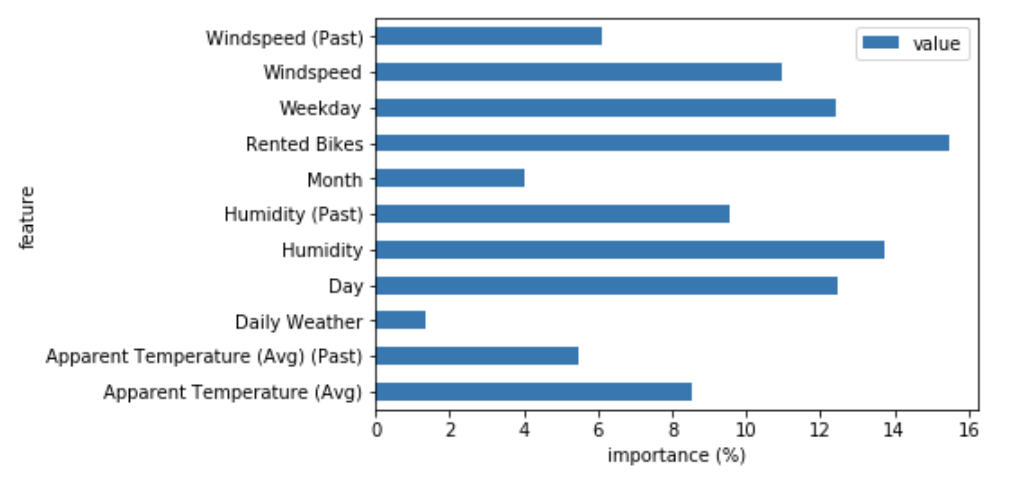
\includegraphics[width=0.8\textwidth]{media/test2_gb}\label{fig:test2_gb}
\captionof{figure}{Test ​2​ features importance: 88.48}\label{fig:test2_gb}
\end{figure}
\begin{figure}[H]
\centering
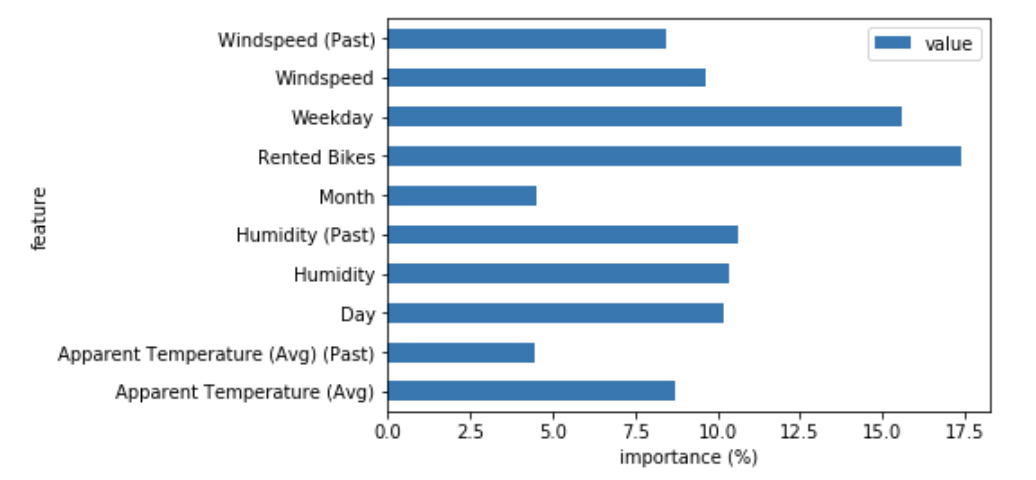
\includegraphics[width=0.8\textwidth]{media/test3_gb}\label{fig:test3_gb}
\captionof{figure}{Test ​3​ features importance: 84.92}\label{fig:test3_gb}
\end{figure}
\begin{figure}[H]
\centering
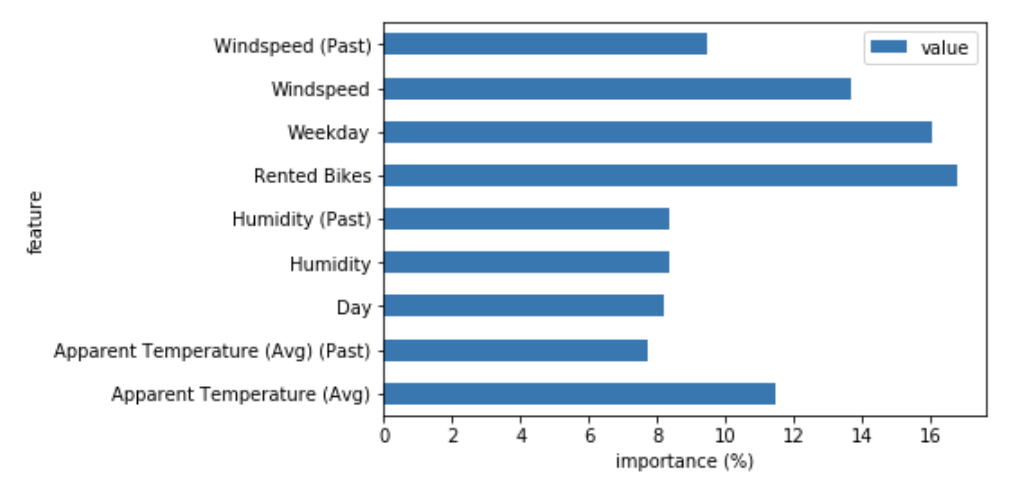
\includegraphics[width=0.8\textwidth]{media/test4_gb}\label{fig:test4_gb}
\captionof{figure}{Test 4 features importance: 76.71}\label{fig:test4_gb}
\end{figure}
\begin{figure}[H]
\centering
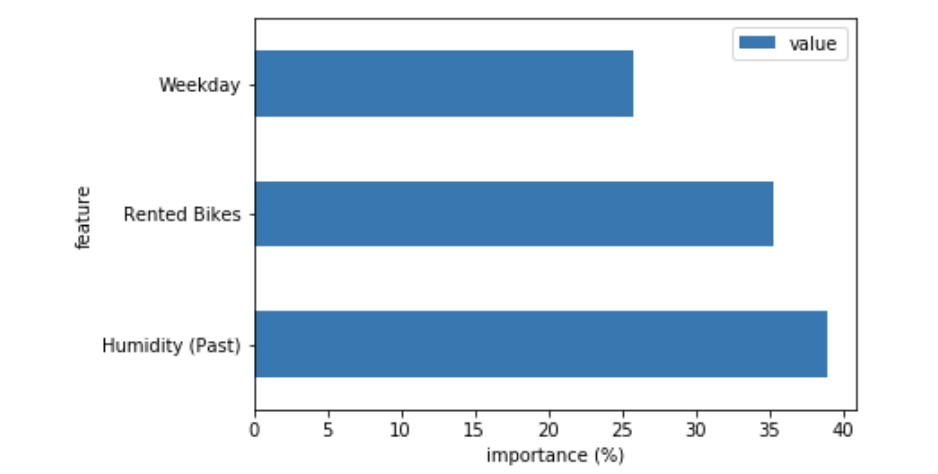
\includegraphics[width=0.8\textwidth]{media/test5_gb}\label{fig:test5_gb}
\captionof{figure}{Test 5 features importance: 63.26}\label{fig:test5_gb}
\end{figure}
The final correlation results are shown in figure \ref{fig:image34} with an RMSE of 63.26.
\begin{figure}[H]
\centering
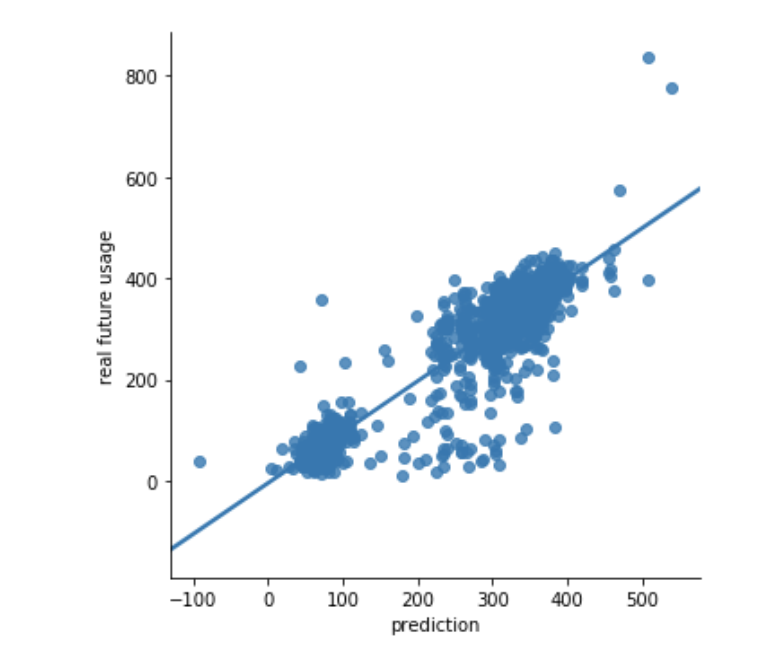
\includegraphics[width=0.6\textwidth]{media/image34}\label{fig:image34}
\captionof{figure}{Data distribution of the actual and predicted data bike usage using Gradient boosted tree regression}\label{fig:image34}
\end{figure}
\begin{figure}[H]
\centering
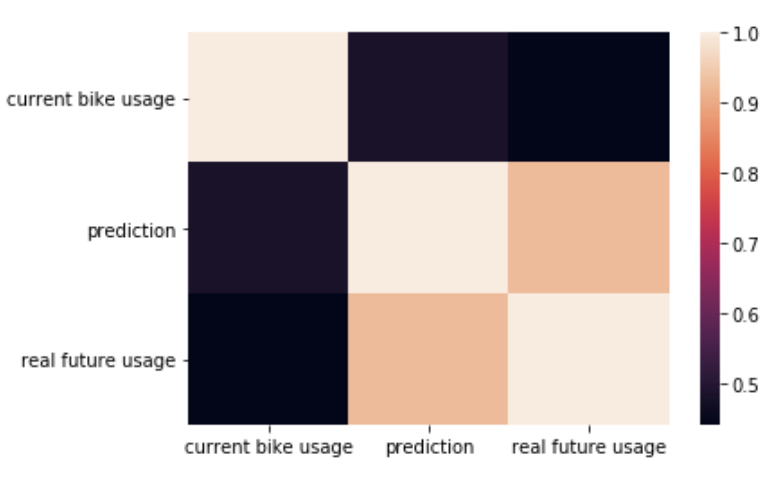
\includegraphics[width=0.8\textwidth]{media/image35}\label{fig:image35}
\captionof{figure}{Heat map correlation plot showing interval value of the regression line (Gradient boosted tree regression)}\label{fig:image35}
\end{figure}
The following test series was implemented by regarding the least used station with a data set consisting of 145 entries.\\\\
\textbf{Decision Tree Regression}\\

The final correlation results are shown in figure \ref{fig:image34} with an RMSE of 11.72.
\begin{figure}[H]
\centering
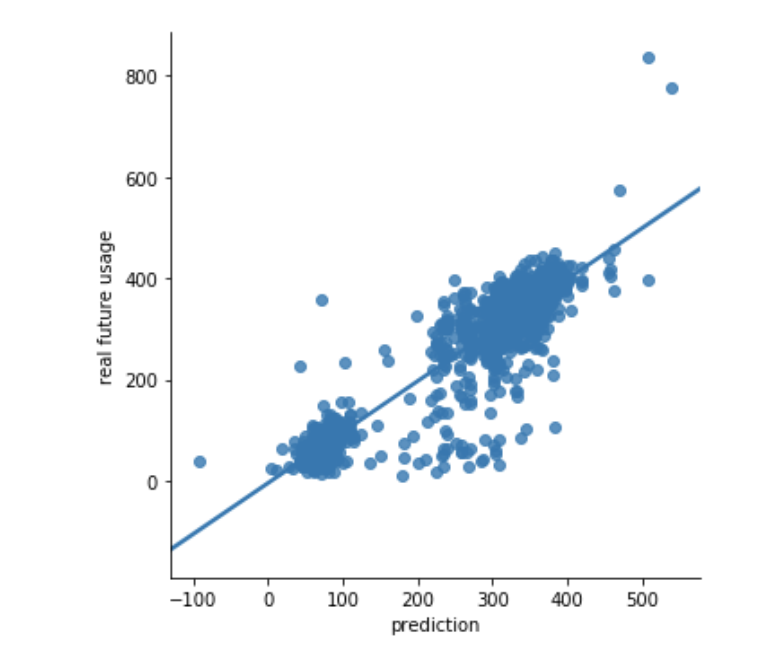
\includegraphics[width=0.6\textwidth]{media/image34}\label{fig:image34}
\captionof{figure}{Data distribution of the actual and predicted data bike usage using Decision Tree Regression}\label{fig:image34}
\end{figure}
\begin{figure}[H]
\centering
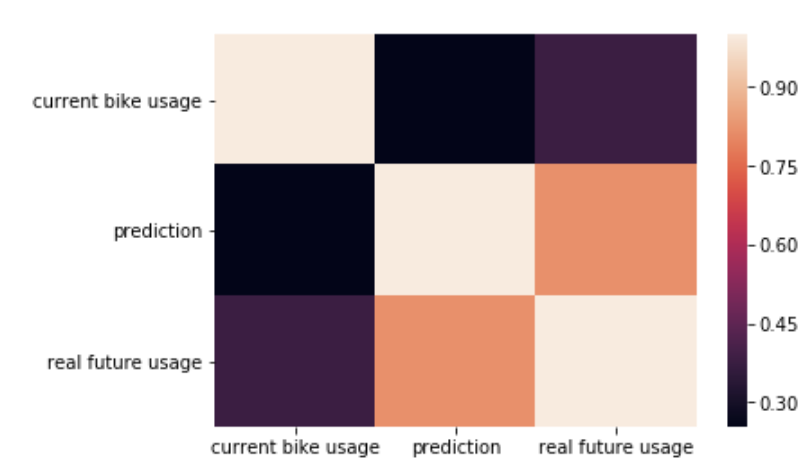
\includegraphics[width=0.8\textwidth]{media/image18}\label{fig:image18}
\captionof{figure}{Heat map correlation plot showing interval value of the regression line (Decision Tree Regression)}\label{fig:image18}
\end{figure}
Figure \ref{fig:anasst4} shows the removed columns and RMSE results.
\begin{figure}[H]
\centering
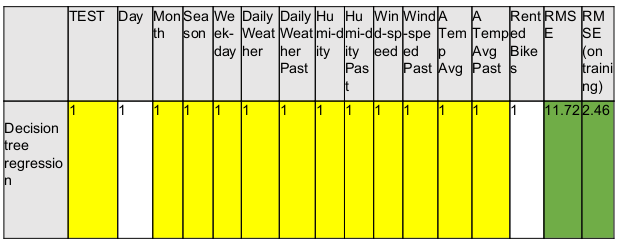
\includegraphics[width=0.8\textwidth]{media/anasst4}\label{fig:anasst4}
\captionof{figure}{Feature evaluation test cases}\label{fig:anasst4}
\end{figure}

\textbf{Random Forest}\\
The final correlation results are shown in figure \ref{fig:image19} with an RMSE of 10.69.
\begin{figure}[H]
\centering
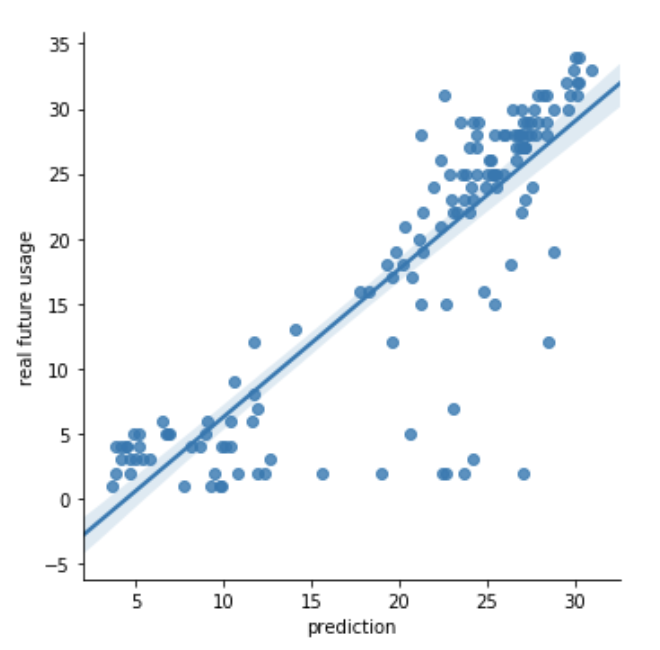
\includegraphics[width=0.6\textwidth]{media/image19}\label{fig:image19}
\captionof{figure}{Data distribution of the actual and predicted data bike usage using Random Forest}\label{fig:image19}
\end{figure}
\begin{figure}[H]
\centering
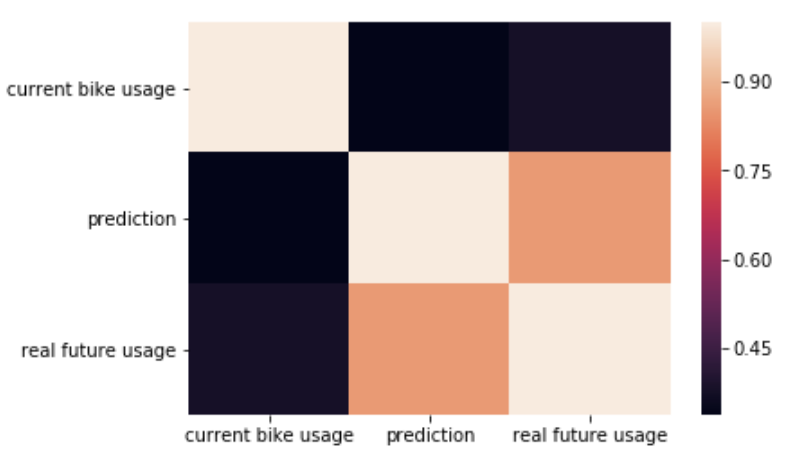
\includegraphics[width=0.8\textwidth]{media/image1a}\label{fig:image1a}
\captionof{figure}{Heat map correlation plot showing interval value of the regression line (Random Forest)}\label{fig:image1a}
\end{figure}
Figure~\ref{fig:anasst4} shows the removed columns and RMSE results.
\begin{figure}[H]
\centering
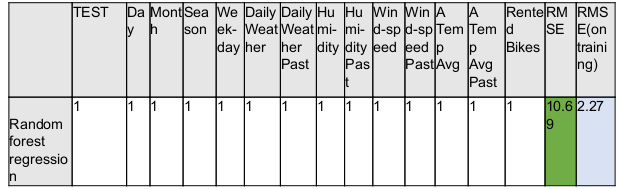
\includegraphics[width=0.8\textwidth]{media/anasst5}\label{fig:anasst5}
\captionof{figure}{Feature evaluation test cases}\label{fig:anasst5}
\end{figure}

\textbf{Gradient boosted tree regression}\\
The final correlation results are shown in figure \ref{fig:image1b} with an RMSE of 11.60.
\begin{figure}[H]
\centering
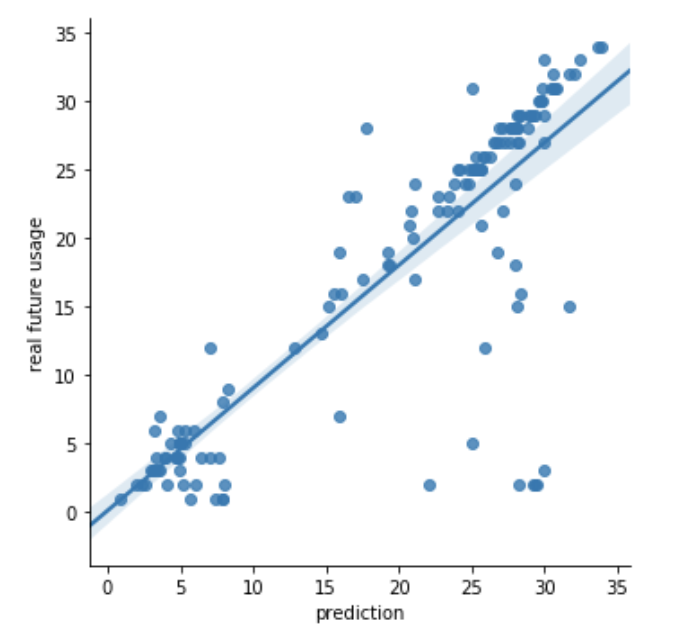
\includegraphics[width=0.6\textwidth]{media/image1b}\label{fig:image1b}
\captionof{figure}{Data distribution of the actual and predicted data bike usage using Gradient boosted tree regression}\label{fig:image1b}
\end{figure}
\begin{figure}[H]
\centering
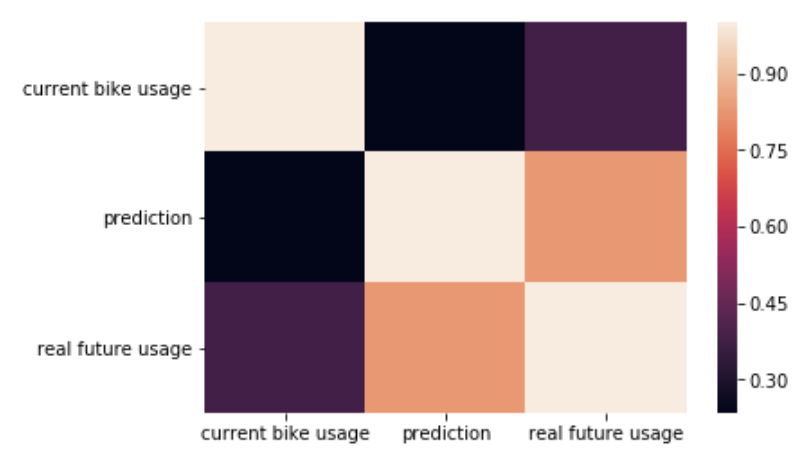
\includegraphics[width=0.8\textwidth]{media/image1c}\label{fig:image1c}
\captionof{figure}{Heat map correlation plot showing interval value of the regression line (Gradient boosted tree regression)}\label{fig:image1c}
\end{figure}
Figure \ref{fig:anasst6} shows the removed columns and RMSE results.
\begin{figure}[H]
\centering
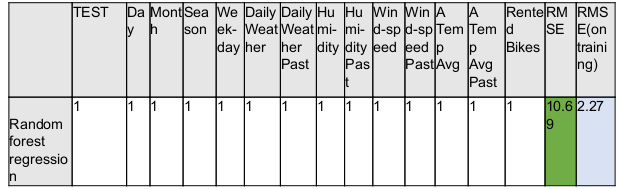
\includegraphics[width=0.8\textwidth]{media/anasst5}\label{fig:anasst6}
\captionof{figure}{Feature evaluation test cases}\label{fig:anasst6}
\end{figure}
\subsection{Modeling (Polynomial Regression)}\label{poly}
Since we don't have a linear relationship between the data, a linear regression will not be helpful.
For example, the regress \glqq Rented Bikes\grqq is not a linear correlation of temperature as even on rainy
days there is slight chance that more people rent a bike than on a sunny day due to a special
holiday. Therefore polynomial regression was a selected machine learning method for the
prediction of rented bikes on a station.\\\\
Polynomial regression belongs to the regression forms \cite{RN9}. In fact, it is just a modified version of a
linear regression. This means the independent variable x and the dependent variable y is modeled
as an nth digress (so-called polynomial) in x \cite{RN9}.\\\\
In a more formal way, the polynomial regression can be expressed as following:
$$Y=\beta_0+\beta_1* x+\beta_2 * x^2 + \beta_3 * x^3 + ... + \beta_n * x^n$$
Where n is the degree of the regression.\\\\
With the Scikit-library in python a data scientist can import the function \glqq PolynomialFeatures\grqq from
\glqq sklearn.preprocessing\grqq which transforms linear data into higher dimensional data. For example
one could apply \glqq poly = PolynomialFeatures(degree = 3)\grqq to get a polynomial
regression in the third dimension. This should improve the accuracy as our underlying data has
no linear relationships but maybe higher dimensional ones. Furthermore, the higher the degree
the better the accuracy should be. Unfortunately the computation time is exponential. A degree of
4 already took several hours to perform and was only slightly better than a regression in the third
dimension.\\\\
The RMSE error on a degree of 4 was around 48,4, which is in comparison to the other tested
ones not really bad but maybe also not best one.\\\\
Figure \ref{fig:figure9_polynomial_features} shows the different plots of each feature and the prediction (rented usage). It turns out
that the feature Season, for example, has no substantial influence on the use of bicycles, whereby
there was apparently an outlier in spring with 800 rented bicycles. It is also becoming apparent
that bicycles are rented more frequently at low wind speeds than at high wind speeds. The average
temperatures between 30 and 70 Fahrenheit are particularly high. Unfortunately, the addition of
the past data has not caused much change in accuracy, as shown in figure \ref{fig:figure9_polynomial_features}.\\\\
Figure \ref{fig:figure10_polynomial_prediction} shows a plot of the tested data (prediction) with the feature \glqq Daily Weather\grqq . The plot looks relatively good, except for a few single outliers at 2 (partly-cloudy-day), the prediction of the
tested data matches the training data.
\begin{figure}[H]
\hspace{-2.8cm}
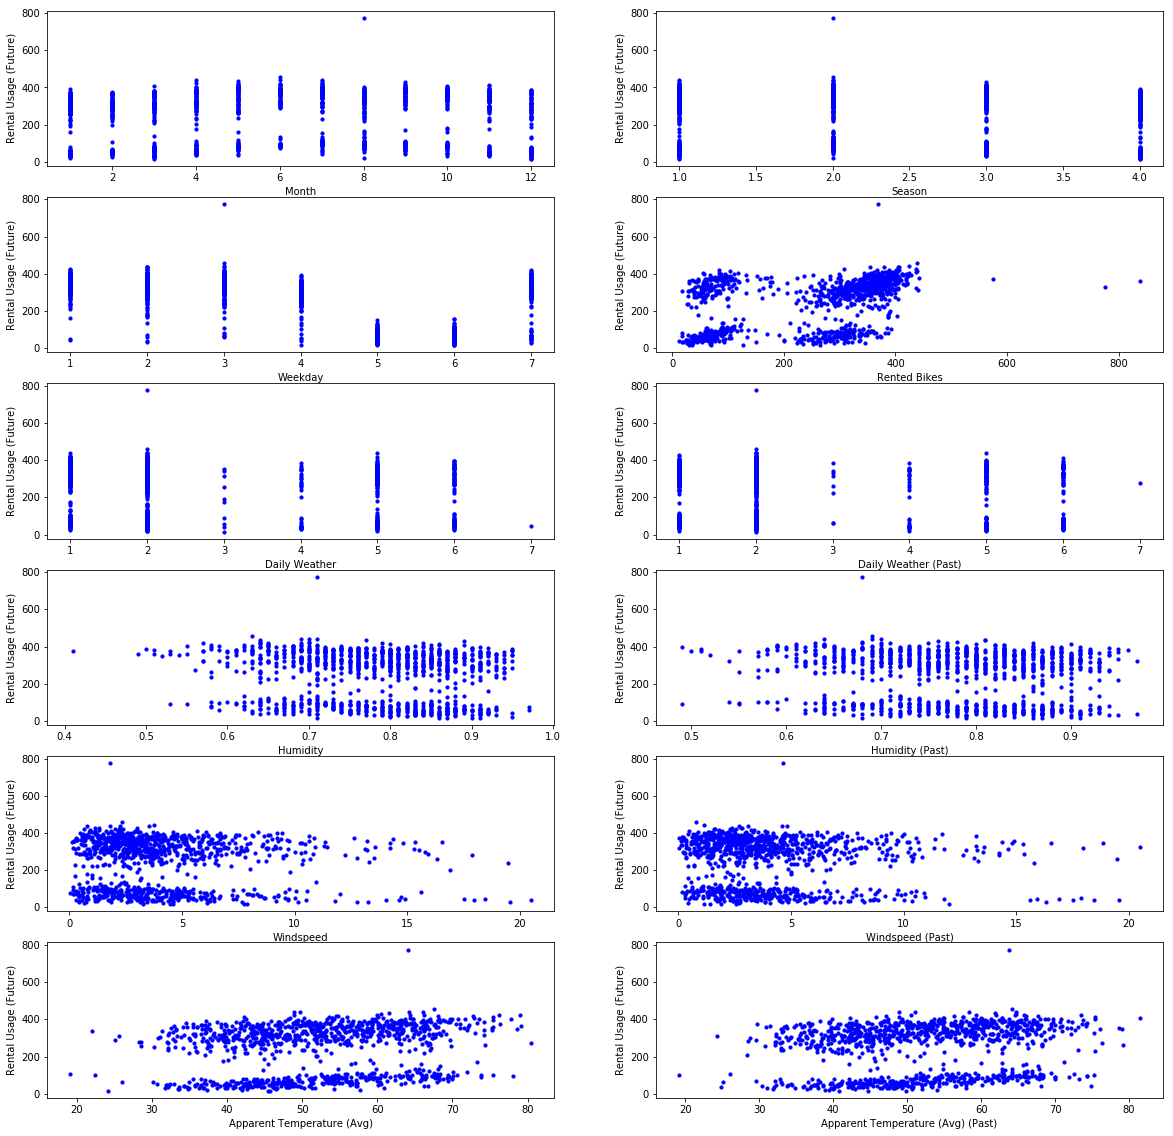
\includegraphics[width=1.4\textwidth]{img/figure9_polynomial_features}\label{fig:figure9_polynomial_features}
\captionof{figure}{Plot of polynomial regression (features)}\label{fig:figure9_polynomial_features}
\end{figure}
\begin{figure}[H]
\hspace{-2.4cm}
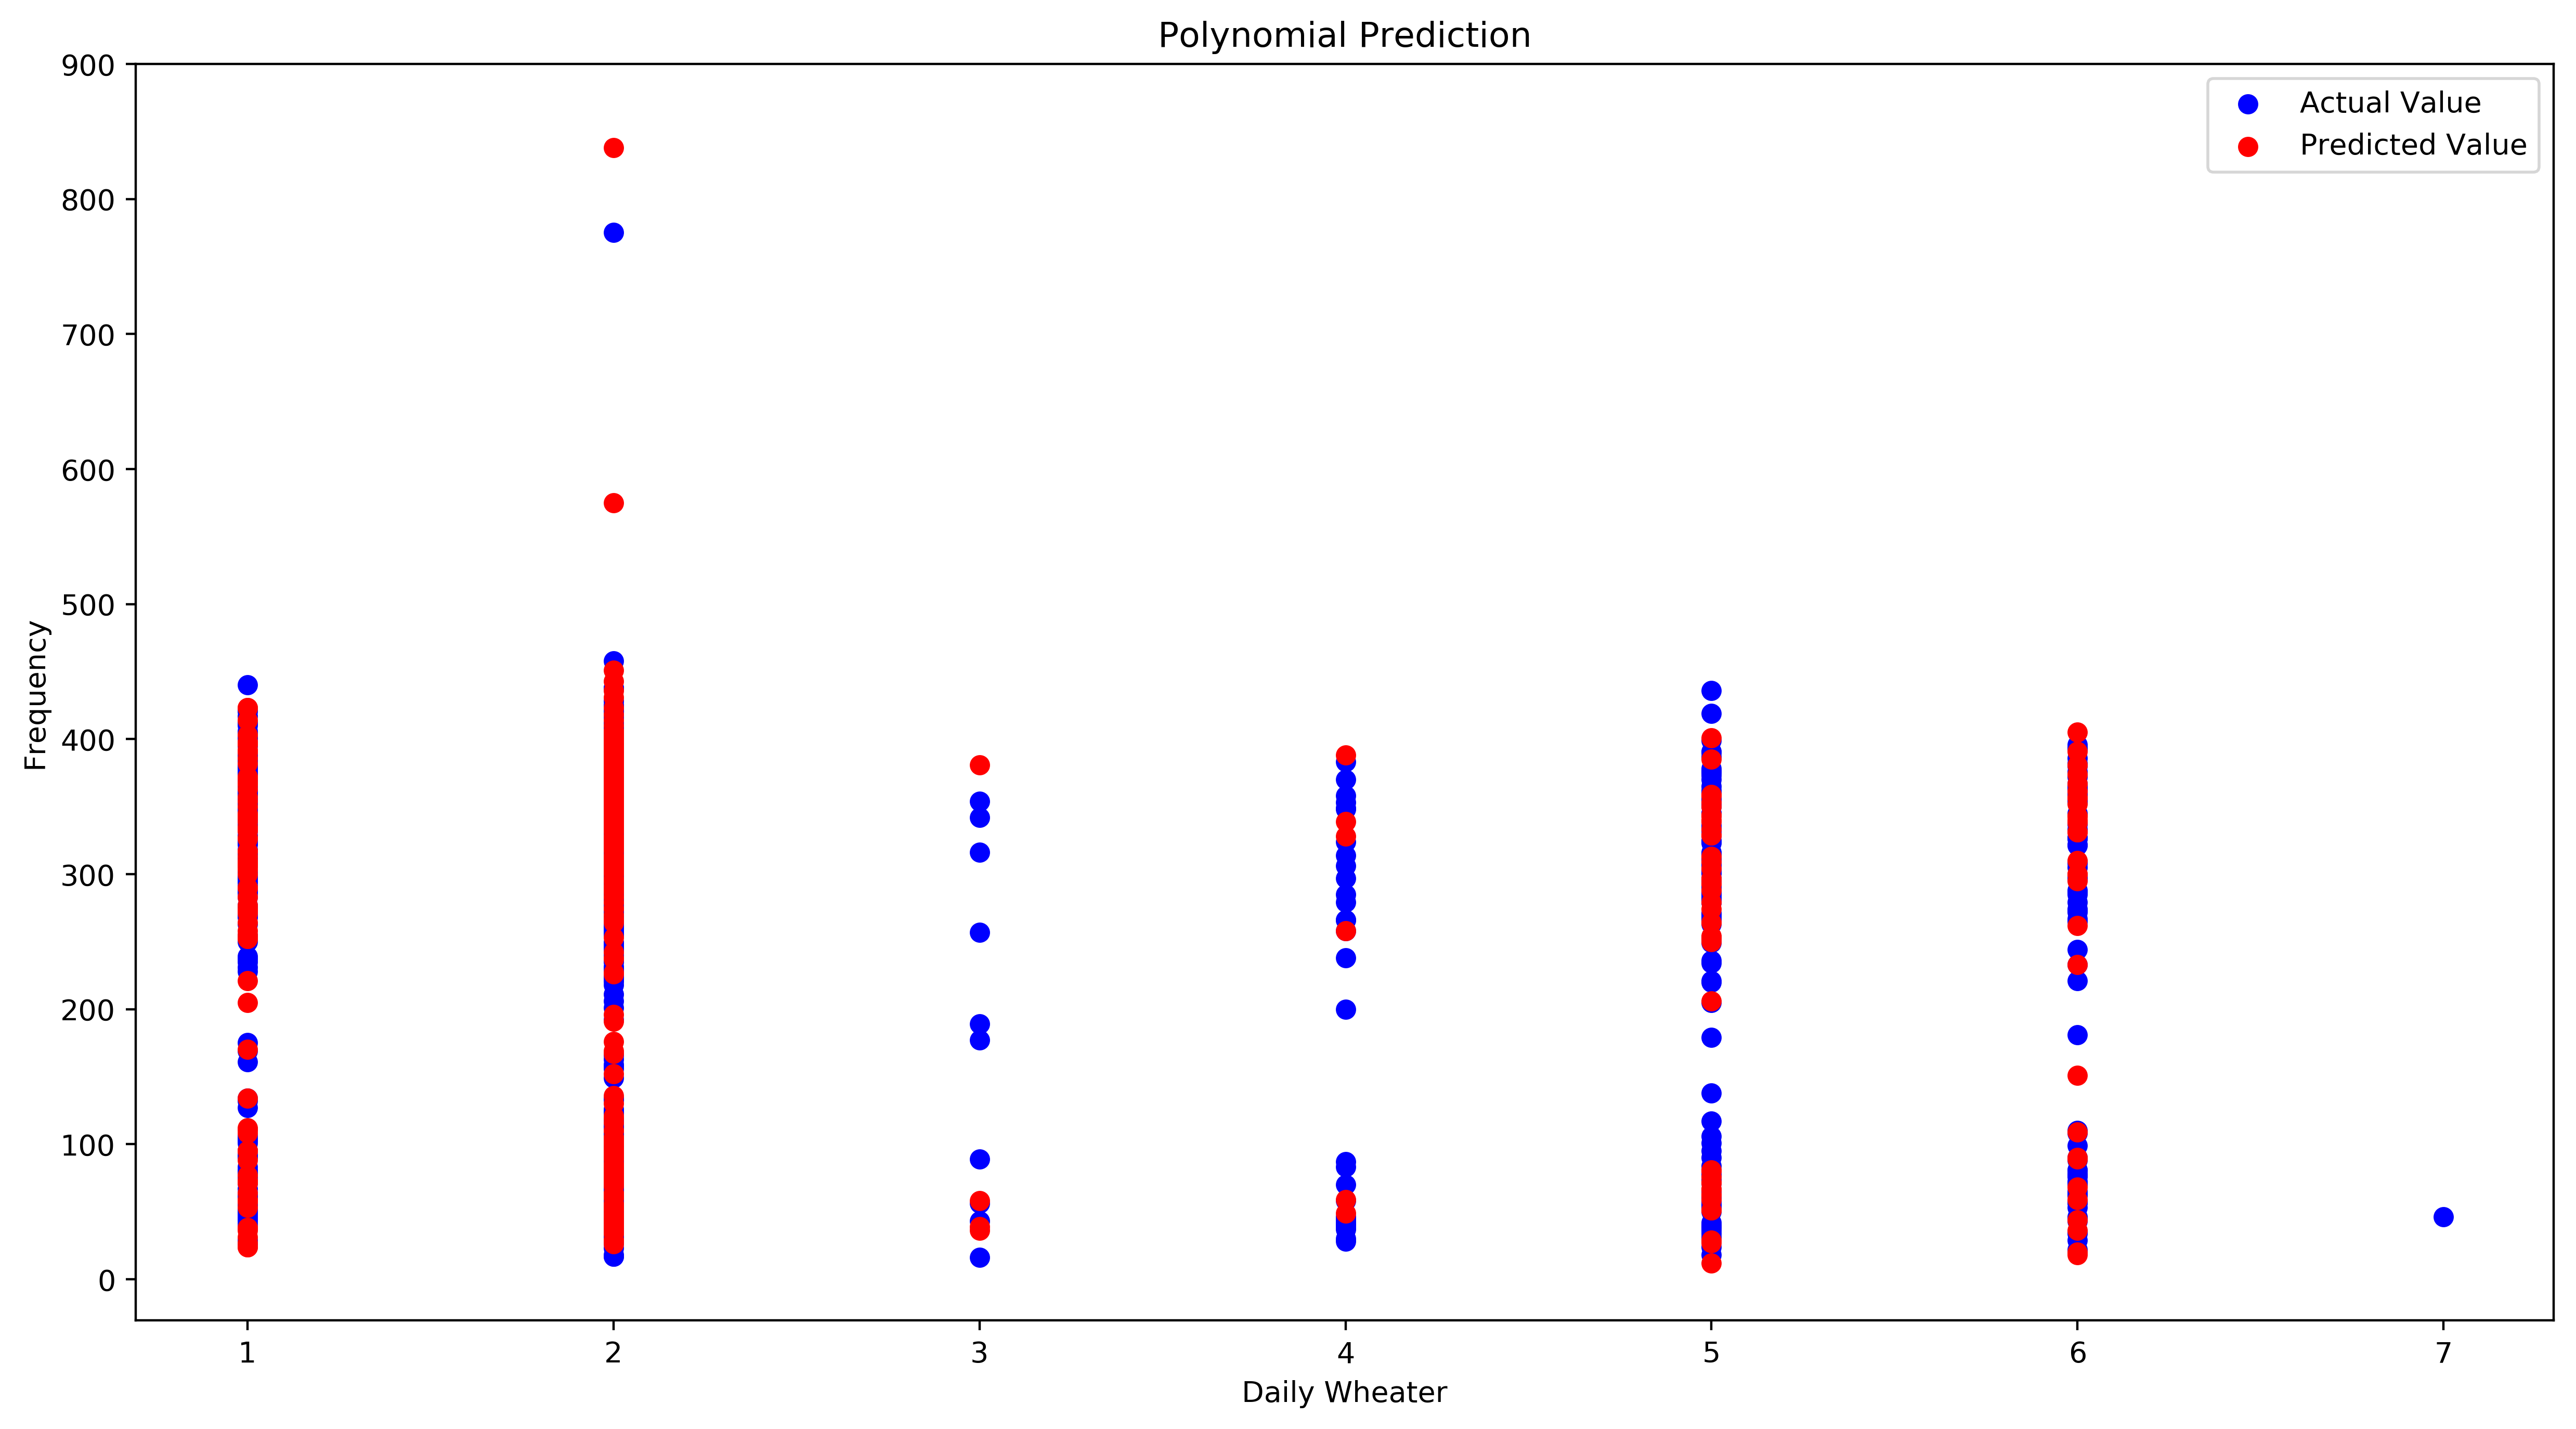
\includegraphics[width=1.3\textwidth]{img/figure10_polynomial_prediction}\label{fig:figure10_polynomial_prediction}
\captionof{figure}{Polynomial Prediction of rental usage on daily weather}\label{fig:figure10_polynomial_prediction}
\end{figure}
